\section{Robovetter Metric Details}
\label{s:metrics}
In this appendix we describe, in detail, each of the Robovetter tests in the order in which they are performed by the Robovetter. See \S\ref{s:robovetter} for an overview of the logic used by the Robovetter.

\subsection{Two Robovetter Detrendings}
As mentioned in \S\ref{abbrev}, for all of the Robovetter tests that require a phased light curve and model fit, we utilize two different detrendings and model fits (named ALT and DV). Every test that is applied to the DV phased light curves is also applied to the ALT detrending, albeit with different thresholds for failure. Failing a test using either detrending results in the TCE being classified as an FP.

In the \kepler{} Pipeline, the DV module produces a harmonic-removed, median-detrended, phased flux light curve, along with a transit model fit \citep{JenkinsKDPH,Wu2010}. However, the harmonic removal software is known to suppress or distort short-period ($\lesssim$ 3 days) signals causing short-period eclipsing binaries with visible secondaries to appear as transiting planets with no visible secondaries \citep{Christiansen2013b}. It can also make variable stars with semi-coherent variability, such as star spots or pulsations, appear as transit-like signals. As an alternative, we implement the ALT detrending method that utilizes the pre-search data conditioned (PDC) time-series light curves and the non-parametric penalized least squares detrending method of \citet{Garcia2010} which includes only the out-of-transit points when computing the filter. This ALT detrending technique is effective at accurately detrending short-period eclipsing binaries and variable stars, i.e., preserving their astrophysical signal.  These ALT detrended light curves are phased and fit with a simple trapezoidal transit model. 

%Thus, we create phased flux light curves via an alternate detrending method that utilizes the pre-search data conditioned (PDC) time-series light curves and the non-parametric penalized least squares detrending method of \citet{Garcia2010}, which includes only the out-of-transit points when computing the filter. These alternately (ALT) detrended light curves are then phased and fit with a simple trapezoidal transit model. This alternate detrending technique is effective at accurately detrending short-period eclipsing binaries and variable stars, i.e., preserving their astrophysical signal. Every test that is applied to the DV phased light curves is also applied to the alternate detrending, albeit with different thresholds for failure. Failing a test using either detrending results in the TCE being classified as an FP.


\subsection{The TCE is the Secondary of an Eclipsing Binary}
\label{s:issecond}
If a TCE under examination is not the first one in a system, the Robovetter checks if there exists a previous TCE with a similar period that was designated as an FP due to a significant secondary (see~\S\ref{sigsecsec}). To compute whether two TCEs have the same period within a given statistical threshold, we employ the period matching criteria of \citet[][see equations 1-3]{Coughlin2014a}, $\sigma_{P}$, where higher values of $\sigma_{P}$ indicate more significant period matches. We re-state the equations here as:

\begin{equation}
\label{peq1}
\Delta P = \frac{P_{A}-P_{B}}{P_{A}}\\
\end{equation}

\begin{equation}
\label{peq2}
\Delta P^{\prime} = \textrm{abs}(\Delta P - \textrm{rint}(\Delta P))\\
\end{equation}

\begin{equation}
\label{peq3}
\sigma_{P} = \sqrt{2}\cdot\textrm{erfcinv}(\Delta P^{\prime})\\
\end{equation}

\noindent where $P_{A}$ is the period of the shorter-period TCE, $P_{B}$ is the period of the longer-period TCE, $\mathrm{rint()}$ rounds a number to the nearest integer, $\mathrm{abs()}$ yields the absolute value, and $\mathrm{erfcinv()}$ is the inverse complementary error function. We consider any value of $\sigma_{P}$ $>$ 3.5 to indicate significantly similar periods.

If the current TCE is (1) in a system that has a previous TCE dispositioned as an FP due to a significant secondary, (2) matches the previous TCE's period with $\sigma_{P}$ $>$ 3.5, and (3) is separated in phase from the previous TCE by at least 2.5 times the transit duration, then the current TCE is considered to be a secondary eclipse. In this case, it is designated as an FP and is classified into both the not transit-like and secondary eclipse FP categories --- a unique combination that can be used to identify secondary eclipses while still ensuring they are not assigned \kepler{} Object of Interest numbers (see \S\ref{koisec}). Note that since the \kepler{} pipeline identifies TCEs in order of their SNR, from high to low, sometimes a TCE identified as a secondary can have a deeper depth than the primary, depending on their relative durations and shapes.

There are two corner cases where we modify the three criteria above. First, it is possible that the periods of two TCEs will meet the period matching criteria, but be different enough to have their relative phases shift significantly over the $\approx$4 year mission duration. Thus, the potential secondary TCE is actually required to be separated in phase by at least 2.5 times the previous TCE's transit duration over the entire mission time frame in order to be labeled as a secondary. Second, the \kepler{} pipeline will occasionally detect the secondary eclipse of an EB at a half, third, or some smaller integer fraction of the orbital period of the system, such that the epoch of the detected secondary coincides with that of the primary. Thus, when a non-1:1 period ratio is detected, we do not impose criteria (3), the phase separation requirement. Note, equations~\ref{peq1}-\ref{peq3} allow for integer period ratios.



\subsection{Not Transit-Like}
\label{nottransitlikesec}

A very large fraction of false positive TCEs have light curves that do not resemble a detached transiting or eclipsing object. These include quasi-sinusoidal light curves from pulsating stars, star spots, and contact binaries, as well as more sporadic light curves due to instrumental artifacts. The first step in the catalog process is to determine whether each TCE is not transit-like. All transit-like \opstce{s} are given \kepler{} Object of Interest (KOI) numbers, which are used to keep track of transit-like systems over multiple \kepler{} pipeline runs. We employ a series of algorithmic tests to reliably identify these not transit-like FP TCEs, as shown by the flowchart in Figure~\ref{robovetter-transitlike-fig}.


\begin{figure*}[ht]
\centering
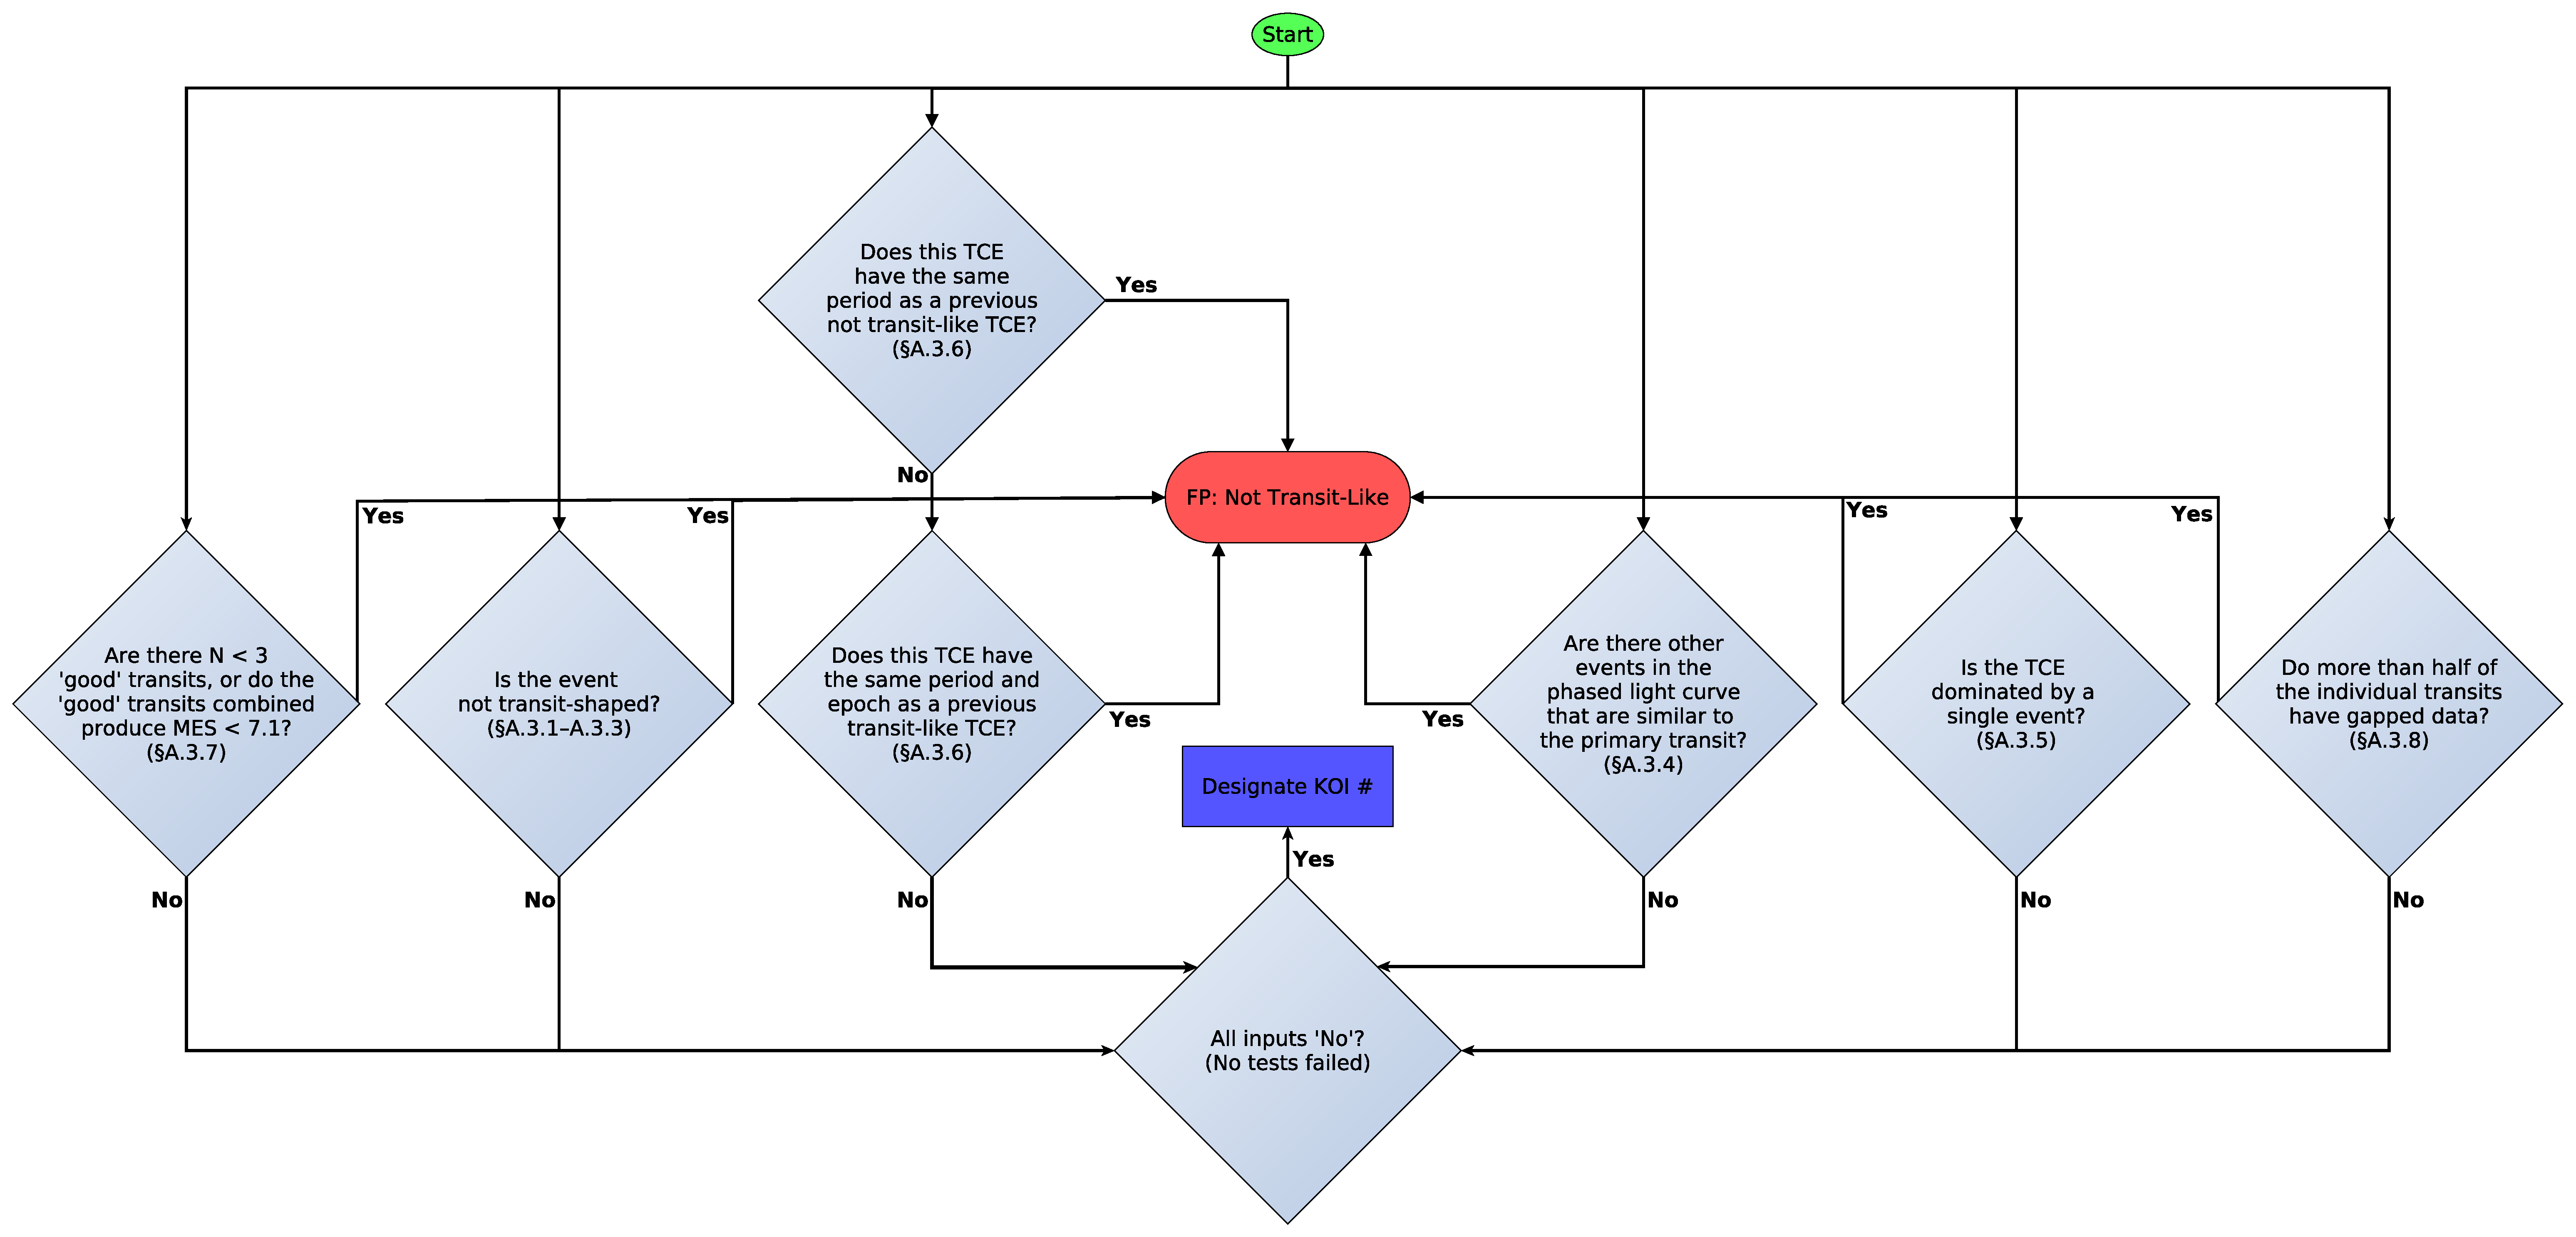
\includegraphics[width=\linewidth]{RoboVetter-Diagram-V4-TransitLike.pdf}
\caption{The not transit-like flowchart of the Robovetter. Diamonds represent ``yes'' or ``no'' decisions that are made with quantitative metrics. If a TCE fails any test (via a ``yes'' response to any decision) then it is dispositioned as a not transit-like FP. If a TCE passes all tests (via a ``no'' response to all decisions), then it is given a KOI number and passed to the significant secondary module (see \S\ref{sigsecsec} and Figure~\ref{robovetter-sigsec-fig}). The section numbers on each decision diamond correspond to the sections in this paper where these tests are discussed.}
\label{robovetter-transitlike-fig}
\end{figure*}


%\subsubsection{Not Transit-Shaped}

%One of the most common false positives in the data set are quasi-sinusoidal shaped light curves, compared to those that are more detached due to a transit or eclipse. Also, individual events can often be due a systematic feature, such as a sudden discontinuity in the light curve. As such, the Robovetter employs tests that detect quasi-sinusoidal light curves and systematics.


\subsubsection{The LPP Metric}
\label{s:lpp}

Many short-period FPs are due to variable stars that exhibit a quasi-sinusoidal phased light curve. We implement the LPP transit-like metric described by \citet{Thompson2015b} to separate those TCEs that show a transit shape from those that do not. This technique bins the TCE's folded light curve and then applies a dimensionality reduction algorithm called Locality Preserving Projections \citep[LPP, ][]{He2004}.  It then measures the average Euclidean distance in these reduced dimensions to the nearest known transit-like TCEs to yield a single number that represents the similarity of a TCE's shape to that of known transits. 

For the DR25 KOI catalog, we deviated slightly from the method described by \citet{Thompson2015b}\footnote{The code is available on Sourceforge here https://sourceforge.net/p/lpptransitlikemetric/}.  The DR24 LPP metric algorithm, when applied to DR25, produced LPP values that were systematically higher for short-period, low-MES TCEs. The transit duration of short period TCEs can be a significant fraction of the orbital period, so when folded and binned these transits have a noticeably different shape. And since we use \injtce{s} as our training set, which has very few short-period examples, there are very few known transits for the algorithm to match to causing large measured distances for these transit event. The trend with MES is rooted in the fact that when the binned light curve has a lower signal-to-noise, it is less likely for two folded light curves to be similar to each other, creating more scatter in the reduced dimensions, and thus increasing the measured distance in those dimensions.  

We reduced these dependencies by altering how we calculate the LPP metric for the DR25 KOI catalog. For our set of known transit-like TCEs, we now use the union of the set of recovered \injtce{s} and set of PCs from the DR24 KOI catalog \citep{Coughlin2016} that were refound as \opstce{s} in DR25. Including these PCs provides more examples at short period. We also changed how the folded light curve was binned. TCEs with lower MES are given wider bins for those cadences near the transit center, while keeping the total number of bins fixed (99 bins total including 41 for the in-transit portion). Finally, we divide these raw LPP values by the 75$^{th}$ percentile of the raw LPP values for the 100 TCEs that are closest in period.  In this way we reduce the period dependence in the LPP metric.  Generally, the resulting LPP metric values lie near to a value of one where values greater than $\approx$ 2 are not transit shaped.  To create the DR25 catalog the Robovetter adopted a threshold of 2.2 for the DV detrending and 3.2 for the ALT detrending.





\subsubsection{Sine Wave Event Evaluation Test}
\label{s:sweetntl}

On occasion, a variable star's variability will have been mostly removed by both the DV and ALT detrendings and will thus appear transit-like. To identify these cases we developed the Sine Wave Event Evaluation Test (SWEET) to examine the PDC data and look for a strong sinusoidal signal at the TCE's period. 

SWEET begins with the PDC data and normalizes each quarter by dividing the time series by the median flux value and subtracting 1.0. Outliers are removed by utilizing a criterion based on the median absolute deviation (MAD). Three different sine curves are fitted to the resulting data, with their periods fixed to half, exactly, and twice the TCE period, with their phase, amplitude, and offset allowed to vary. Of the three fits, the one with the highest signal-to-noise ratio, defined as the amplitude divided by its error, is chosen as the strongest fit. If a TCE has a SWEET signal-to-noise ratio greater than 50, an amplitude greater than the TCE transit depth in both the DV and ALT detrendings, and has a period less than 5.0 days, it fails as not transit-like.

% Can provide exact outlier rejection formula if desired, but seemed unnecessary



\subsubsection{TCE Chases}
\label{s:tcechases}

In \S\ref{s:chases} we describe a individual transit metric called Chases that assesses the detection strength of individual transit events relative to other signals nearby in time. TCE Chases takes the median value of these individual transit measurements.  When the median value is less than 0.8 the TCE fails as not-transit-like.  As with the individual Chases metric, TCE Chases is only calculated when the TCE has five or fewer transit events contributing to the signal.  With more than five transit events, the individual transit events are not expected to be statistically significant, and the assumptions of the Chases metric no longer apply.


\subsubsection{The Model-Shift Uniqueness Test}
%\label{notuniquetcesec}
\label{s:ms}

If a TCE under investigation is truly a PC, there should not be any other transit-like events in the light curve with a depth, duration, and period similar to the primary signal, in either the positive or negative flux directions, i.e., the transit event should be unique in the phased light curve. Many false positives are due to quasi-sinusoidal signals (see \S\ref{tcesec}) and thus are not unique in the phased light curve. In order to identify these cases, we developed a ``model-shift uniqueness test'' and used it extensively for identifying false positives in the Q1--Q12 \citep{Rowe2015a}, Q1--Q16 \citep{Mullally2015cat}, and DR24 \citep{Coughlin2016} planet candidate catalogs.

See \S3.2.2 of \citet{Rowe2015a} and page 23 of \citet{Coughlin2017b} for figures and a detailed explanation of the ``model-shift uniqueness test''. Briefly, after removing outliers, the best-fit model of the primary transit is used as a template to measure the best-fit depth at all other phases. The deepest event aside from the primary (pri) transit event is labeled as the secondary (sec) event, the next-deepest event is labeled as the tertiary (ter) event, and the most positive (pos) flux event (i.e., shows a flux brightening) is labeled as the positive event. The significances of these events ($\sigma_{\rm Pri}$, $\sigma_{\rm Sec}$, $\sigma_{\rm Ter}$, and $\sigma_{\rm Pos}$) are computed assuming white noise as determined by the standard deviation of the light curve residuals. Also, the ratio of the red noise (at the timescale of the transit duration) to the white noise ($F_{\rm Red}$) is computed by examining the standard deviation of the best-fit depths at phases outside of the primary and secondary events.  

When examining all events among all TCEs, assuming Gaussian noise, the minimum threshold for an event to be considered statistically significant is given by

\begin{equation}
    FA_{1} = \sqrt{2}\cdot \textrm{erfcinv}\left(\frac{T_{\rm dur}}{P \cdot N_{\rm TCEs}}\right)
\end{equation}

\noindent where $T_{\rm dur}$ is the transit duration, $P$ is the period, and N$_{\rm TCEs}$ is the number of TCEs examined. (The quantity $P$/$T_{\rm dur}$ represents the number of independent statistical tests for a single target.) When comparing two events from the same TCE, the minimum difference in their significances in order to be considered distinctly different is given by

\begin{equation}
    FA_{2} = \sqrt{2}\cdot \textrm{erfcinv}\left(\frac{T_{\rm dur}}{P}\right)
\end{equation}

\noindent We compute the following quantities to use as decision metrics:

\begin{equation}
    MS_{1} = FA_{1} - \sigma_{\rm Pri}/F_{\rm Red}
\end{equation}

\begin{equation}
    MS_{2} = FA_{2} - (\sigma_{\rm Pri} - \sigma_{\rm Ter})
\end{equation}

\begin{equation}
    MS_{3} = FA_{2} - (\sigma_{\rm Pri} - \sigma_{\rm Pos})
\end{equation}

In the Robovetter, we disposition a TCE as a not transit-like FP if either $MS_{1}$~$>$~1.0, $MS_{2}$~$>$~2.0, or $MS_{3}$~$>$~4.0 in the DV detrending, or if either $MS_{1}$~$>$~-3.0, $MS_{2}$~$>$~1.0, or $MS_{3}$~$>$~1.0 in the ALT detrending. These criteria ensure that the primary event is statistically significant when compared to the systematic noise level of the light curve, the tertiary event, and the positive event, respectively. We also fail TCEs as not transit-like if $\sigma_{\rm Pri}$ exactly equals zero in both the DV and ALT detrendings. A vale of zero indicates that the fit failed for both detrendings, and suggests that something is fundamentally flawed with the TCE.


\subsubsection{Dominated by Single Event}
\label{s:sesmes}

The depths of individual transits of planet candidates should be equal to each other, and thus assuming constant noise levels, the SNR of individual transits should be nearly equivalent as well. In contrast, most of the long-period FPs that result from three or more equidistant systematic events are dominated in SNR by one event. The \kepler{} pipeline measures detection significance via the Multiple Event Statistic (MES), which is calculated by combining the Single Event Statistic (SES) of all the individual events that comprise the TCE --- both the MES and SES are measures of SNR. Assuming all individual events have equal SES values,

\begin{equation}
{\rm MES} = \sqrt{N_{\rm Trans}} \cdot {\rm SES}
\end{equation}

\noindent where $N_{\rm Trans}$ is the number of transit events that comprise the TCE. Thus, SES/MES = 0.577 for a TCE with three transits, and less for a greater number of transits. 

If the largest SES value of a TCE's transit events, ${\rm SES}_{\rm Max}$, divided by the MES is much larger than 0.577 (regardless of the number of transits), this indicates that one of the individual events dominates when calculating the SNR.

In the Robovetter, for TCEs with periods greater than 90 days, if ${{\rm SES}_{\rm Max} / {\rm MES} > 0.8}$ it is dispositioned as a not transit-like FP. The period cutoff of 90 days is applied because short-period TCEs can have a large number of individual transit events, which dramatically increases the chance of one event coinciding with a large systematic feature, thus producing a large ${{\rm SES}_{\rm Max} / {\rm MES}}$ value despite being a valid planetary signal.

% The value of 0.8 was empirically chosen based on the results of transit injection (\S\ref{injectsec}) to reject a minimal number of valid planetary candidates, accounting for natural deviations of SES values due to light curve systematics and changes in local noise levels. 


\subsubsection{Previous TCE With Same Period}
\label{s:sameperiod}
Most quasi-sinusoidal FPs produce multiple TCEs at the same period, or at integer ratios of each other. If a TCE in a system has been declared as not transit-like due to another test, it is logical that all subsequent TCEs in that system at the same period, or ratios thereof, should also be dispositioned not transit-like. Thus, we match the period of a given TCE to all previous not transit-like FPs via equations~\ref{peq1}-\ref{peq3}. If the current TCE has a period match with $\sigma_{P}$ $>$ 3.25 to a prior not transit-like FP, it is also dispositioned as a not transit-like FP.

Similarly, some TCEs are produced that correspond to the edge of a previously identified transit-like TCE in the system. This often results when the previous TCE corresponding to a transit or eclipse is not completely removed prior to searching the light curve for another TCE. Thus, we match the period of a given TCE to all previous transit-like TCEs via equations~\ref{peq1}-\ref{peq3}.  If the current TCE has a period match with $\sigma_{P}$ $>$ 3.25 to a prior transit-like FP, and the two epochs are separated in phase by less than 2.5 transit durations, the current TCE is dispositioned as a not transit-like FP. For clarity, we note that it is sometimes possible that the periods of two TCEs will meet the period matching criteria, but be different enough to have their epochs shift significantly in phase over the $\sim$4 year mission duration. Thus, if they are separated in phase by less than 2.5 transit durations at any point in the mission time frame, the current TCE is dispositioned as a not transit-like FP.



\subsubsection{Individual Transit Metrics}
\label{s:indivtrans}
A new approach implemented in DR25 is to examine individual transit events for each TCE and determine if they are transit-like. After rejecting these "bad" transit events, we check if either

\begin{itemize}
\item There are less than 3 "good" events left
\item The re-computed MES using only `good' events is $<$ 7.1
\end{itemize}

\noindent If either of these conditions are met, then the TCE is failed as not transit-like. This is in line with the \kepler{} mission requirement of at least three valid transit events with a MES~$\ge$~7.1 in order to generate a TCE. In the following subsections we list the various tests we apply to each individual transit event.


\paragraph{Rubble -- Missing Data}
\label{s:rubble}
A number of TCEs from the \kepler{} pipeline are based on transit events that are missing a significant amount of data either in-transit or just before and/or after. These tend to be false positives that are triggering on edges of gaps, or cases were a large amount of data has been removed and a TCE is being created from the residuals of previous TCEs in the system. We thus devised the Rubble metric to clean-up these fragments from the TCE list. The Rubble value for each individual transit is computed by dividing the number of \Kepler\ cadences that are available in the DV time series by the number of cadences expected across two transit durations given \Kepler's regular 29.42\,min cadence and the transit duration provided by the DV fit. If the Rubble value for the transit falls below threshold, then that transit is not counted as a valid transit. We adopted a threshold value of 0.5 to generate the DR25 KOI Catalog.


\paragraph{Marshall -- Transit Shape}
\label{s:marshall}
In the DR24 KOI Catalog, \citet{Coughlin2016} used the Marshall algorithm \citep{Mullally2016} to identify and reject false alarm TCEs caused by short period transients in the data. Marshall fits the proposed transit with models of various transients and uses a Bayesian Information Criterion (BIC) to decide which model is the best explanation for the data. Simulations in \citet{Mullally2016} showed that Marshall was 95\% complete for TCEs with periods $>150$\,days and correctly rejected 66\% of simulated artifact events. The limit on Marshall's effectiveness at eliminating false alarms was that it used a parabola to describe the out-of-transit flux, which failed to capture much of the real observed stellar variability. To ensure high completeness, Marshall was tuned to prevent a variable continuum from causing true transits to be rejected, at the cost of a lower effectiveness.

For the DR25 KOI catalog, we use a Gaussian Process approach \citep[GP,][]{Rasmussen10} to provide an improved continuum model and increase our effectiveness, while maintaining our high completeness. Briefly, our approach aims to model the covariance in the light curve to better fit the trends in our data.
A similar approach was used by \citet{ForemanMackey16} to model single transits due to very long period planets ($P > 1000$\,days).

Our procedure is as follows. For each individual proposed transit event, we select a snippet of PDC data 30 times the reported transit duration centered on the event. Where the event happens near the start (or end) of a quarter, we take a snippet of similar length anchored at the start (or end) of the quarter. We use the \emph{George} package \citep{Ambikasaran14} to fit the covariance of the out-of-transit flux with an exponential squared function, $ {\mathrm{Cov(\delta t})} = A \exp{ (\delta t/\ell)^2}$, where $A$ and $\ell$ are tunable parameters. 

We next fit four models to the entire snippet.

\begin{equation}
\left.\begin{aligned}
G(t | A, \ell) + y_0 \\
G(t | A, \ell) + y_0 + S(t)\\
G(t | A, \ell) + y_0 + S(t)(1 - \exp{\beta t})\\
G(t | A, \ell) + y_0 + S(t - \tau/2) - S(t + \tau/2) 
\end{aligned}\right.
\label{e:marshall}
\end{equation}

\noindent
where $G$ is the Gaussian Process model with the tunable parameters held fixed to those found earlier, and $y_0$ is a constant offset. $S(t)$ is given by

\begin{equation}
S(t) = \frac{d}{1 + e^{-\gamma (t-t_0)} }
\end{equation}

\noindent
where $d$ and $t_0$ are tunable parameters and $\gamma$ is a positive constant. This function, known as a sigmoid (or logistic) function, has asympotes of 0 for $t<<t_0$, and d for $t>>t_0$. The function transitions quickly, but smoothly, between the two states near $t=t_0$, where it takes on a value of d/2. 

% I think that gamma, as well as the sign of the exponential term in the  denominator should be positive. The function approaches zero as t - t0 approaches negative infinity, and approaches d as t - t0 approaches infinity.
By using a sigmoid and avoiding the discontinuities present in the models used by the original Marshall algorithm \citep{Mullally2016} we can use the L-BFGS-B algorithm \citep{Byrd95} available in the Scipy package \footnote{\url{www.scipy.org}} instead of the less robust Nelder-Mead.

The second function in equation \ref{e:marshall} models a discrete jump in the data. We fit this model seeded with a negative-going dip at the predicted time of ingress, and also with a positive-going spike at the predicted egress, as we see both types of features in \Kepler\ data. The third model fits a Sudden Pixel Sensitivity Drop (SPSD) event, probably caused by a cosmic ray hit on the detector. The last model approximates a box transit. By varying the parameter $\gamma$ we could in principle model transit ingress and egress, but find that extra degree of freedom is not necessary to fit the low signal-to-noise events of most concern.

For each transit the Marshall method returns the BIC score, the preferred model, and the difference between the BIC scores of the preferred model and the sigmoid box fit.  A transit is considered sufficiently bad when this difference (also known as the Marshall score) exceeds a particular threshold, as with the original Marshall algorithm.  However, in a few cases the Gaussian process fails and yields extremely large, unbelievable BIC values. In these cases the transit is set to always pass.  Also, for low MES transits, the expected SES of a transit is sufficiently low that Marshall will be unable to distinguish between the ``no transit" model and a low signal-to-noise transit.  Because of this the Robovetter declares a specific transit is not valid if all of the following criteria are met:

\begin{itemize}
\item The BIC score of the best-fitting non-transit model is at least 10 lower than the BIC of the transit-model
\item The BIC score of the best-fitting non-transit model is less than 1.0E6
\item Either MES/$\sqrt{\textrm{N}_{\textrm{RealTrans}}}$~$>$~4.0 or the lowest BIC model is for the constant offset model, 
\end{itemize}

Note, N$_{\textrm{RealTrans}}$ is the total number of observed transit events for the TCE. The Marshall code used for the DR25 KOI catalog is available on sourceforge\footnote{ \url{https://sourceforge.net/projects/marshall/}}.


\paragraph{Chases -- SES artifacts}
\label{s:chases}

The Chases metric was developed to chase-down non-transit like events on long period, low MES TCEs. Qualitatively, the metric mimics the human vetting preference to classify a TCE as a PC when individual transit events "stand-out" as a unique, transit-like signal from a visual inspection of the \kepler\ flux time-series data.  In order to quantify this human vetting preference, we developed the the Chases algorithm. Chases uses the SES time series generated by the TPS module of the \kepler\ pipeline \citep{JenkinsKDPH}.  The SES time series measures the significance of a transit signal centered on every cadence.  Details of calculating the SES time series is given in \citet{Jenkins2002a} and illustrative examples are given in \citet{Tenenbaum2012}. A transit produces a peak in the SES time series (as do systematic signals). TPS searches the SES time series for equally spaced peaks indicative of a series of transits. The series of individual peaks in the SES time series are combined to form the MES employed as the primary threshold for detecting a transit signal \citep{Jenkins2002a,Twicken2016,JenkinsKDPH}.  


The Chases metric quantifies how well the SES peaks contributing to a TCE approximate the expected shape and significance (relative to neighboring data) of a bona fide transit signal.  Figure~\ref{fig:chases1} shows the detrended flux time series (upper panel) and the corresponding SES time series (lower panel) for a clear single transit event contributing to the TCE detection of K03900.01 on target KIC~11911580.  The flux time series, with a very clear decrement during in-transit cadences (orange points), has the archetypal SES time series of a strong central peak with two low-amplitude, symmetric side troughs (caused by the way TPS uses wavelets to modify the model transits when calculating the SES, see \citealt{JenkinsKDPH}). 

The Chases metric for an individual transit event is formulated by identifying the maximum SES value for cadences in transit, $SES_{\rm max}$ (in Figure~1, $SES_{\rm max}\sim20$).  Next, excluding cadences within 1.5$\tau_{\rm dur}$ of mid transit, where $\tau_{\rm dur}$ is the detected transit duration, the SES time series is searched for $\Delta_{t}$, the temporally closest feature to mid transit in the absolute value of the SES time series, $\lvert SES \rvert$. A feature is defined as when  $\lvert SES \rvert>f\, SES_{\rm max}$, where $f$ represents a tunable fraction of the peak in the SES time series.  Finally, we define a maximum window $\Delta_{tmax}=P_{orb}/10$ with which to search for a comparable peak in $\lvert SES \rvert$, and form the final Chases metric for an individual transit event as $C_{i} = {\rm min}(\Delta_{t},\Delta_{tmax})/\Delta_{tmax}$.  

A value of $C_{i}=1$ indicates that there is no comparable peak/trough in the SES time series within $f$ of $SES_{\rm max}$ over the interval $\Delta_{tmax}$ of the transit signal.  Thus, $Ch_{i}=1$ is consistent with a unique, transit-like signal.  A value of $Ch_{i}\sim0$ indicates that a comparable strength feature is present in the SES time series temporally close to the transit event, and is consistent with the human vetting tendency to dismiss such signals as spurious.  Figure~\ref{fig:chases2} shows an example of a spurious TCE detection on the target KIC 11449918.  The target is on a detector suffering from elevated levels of the "rolling-band" image artifacts as described in \S\ref{s:skye}.  The neighboring peak of comparable strength in the SES time series would result in $Ch_{i}\sim0$ for this individual transit event.  The Chases metric is also sensitive to the shape of the transit signal as illustrated in Figure~\ref{fig:chases3}. The SPSD shown in Figure~\ref{fig:chases3} is a spurious instrumental signal with an asymmetric shape. Because Chases uses the absolute value of the SES, $Ch_{i}\sim0$ for these types of events.

%A spurious instrumental signal encountered with the \kepler\ detectors is the SPSD shown in Figure~\ref{fig:chases3}.  Using $\lvert SES \rvert$ in formulating the Chases metric allows such asymmetric profiles to be identified with low $Ch_{i}$ values.

For each TCE with five or fewer transit events contributing to the signal, $Ch_{i}$ is calculated for every transit event.  With more than five transit events, the individual transit events are not expected to be statistically significant, and the assumptions of the Chases metric no longer apply. The individual transit event $Ch_{i}$ values were used to recalculate the MES (see \S\ref{s:indivtrans}). Transit events with $Ch_{i}<0.01$ were excluded from the Robovetter's MES calculation.

\begin{figure}[htb]
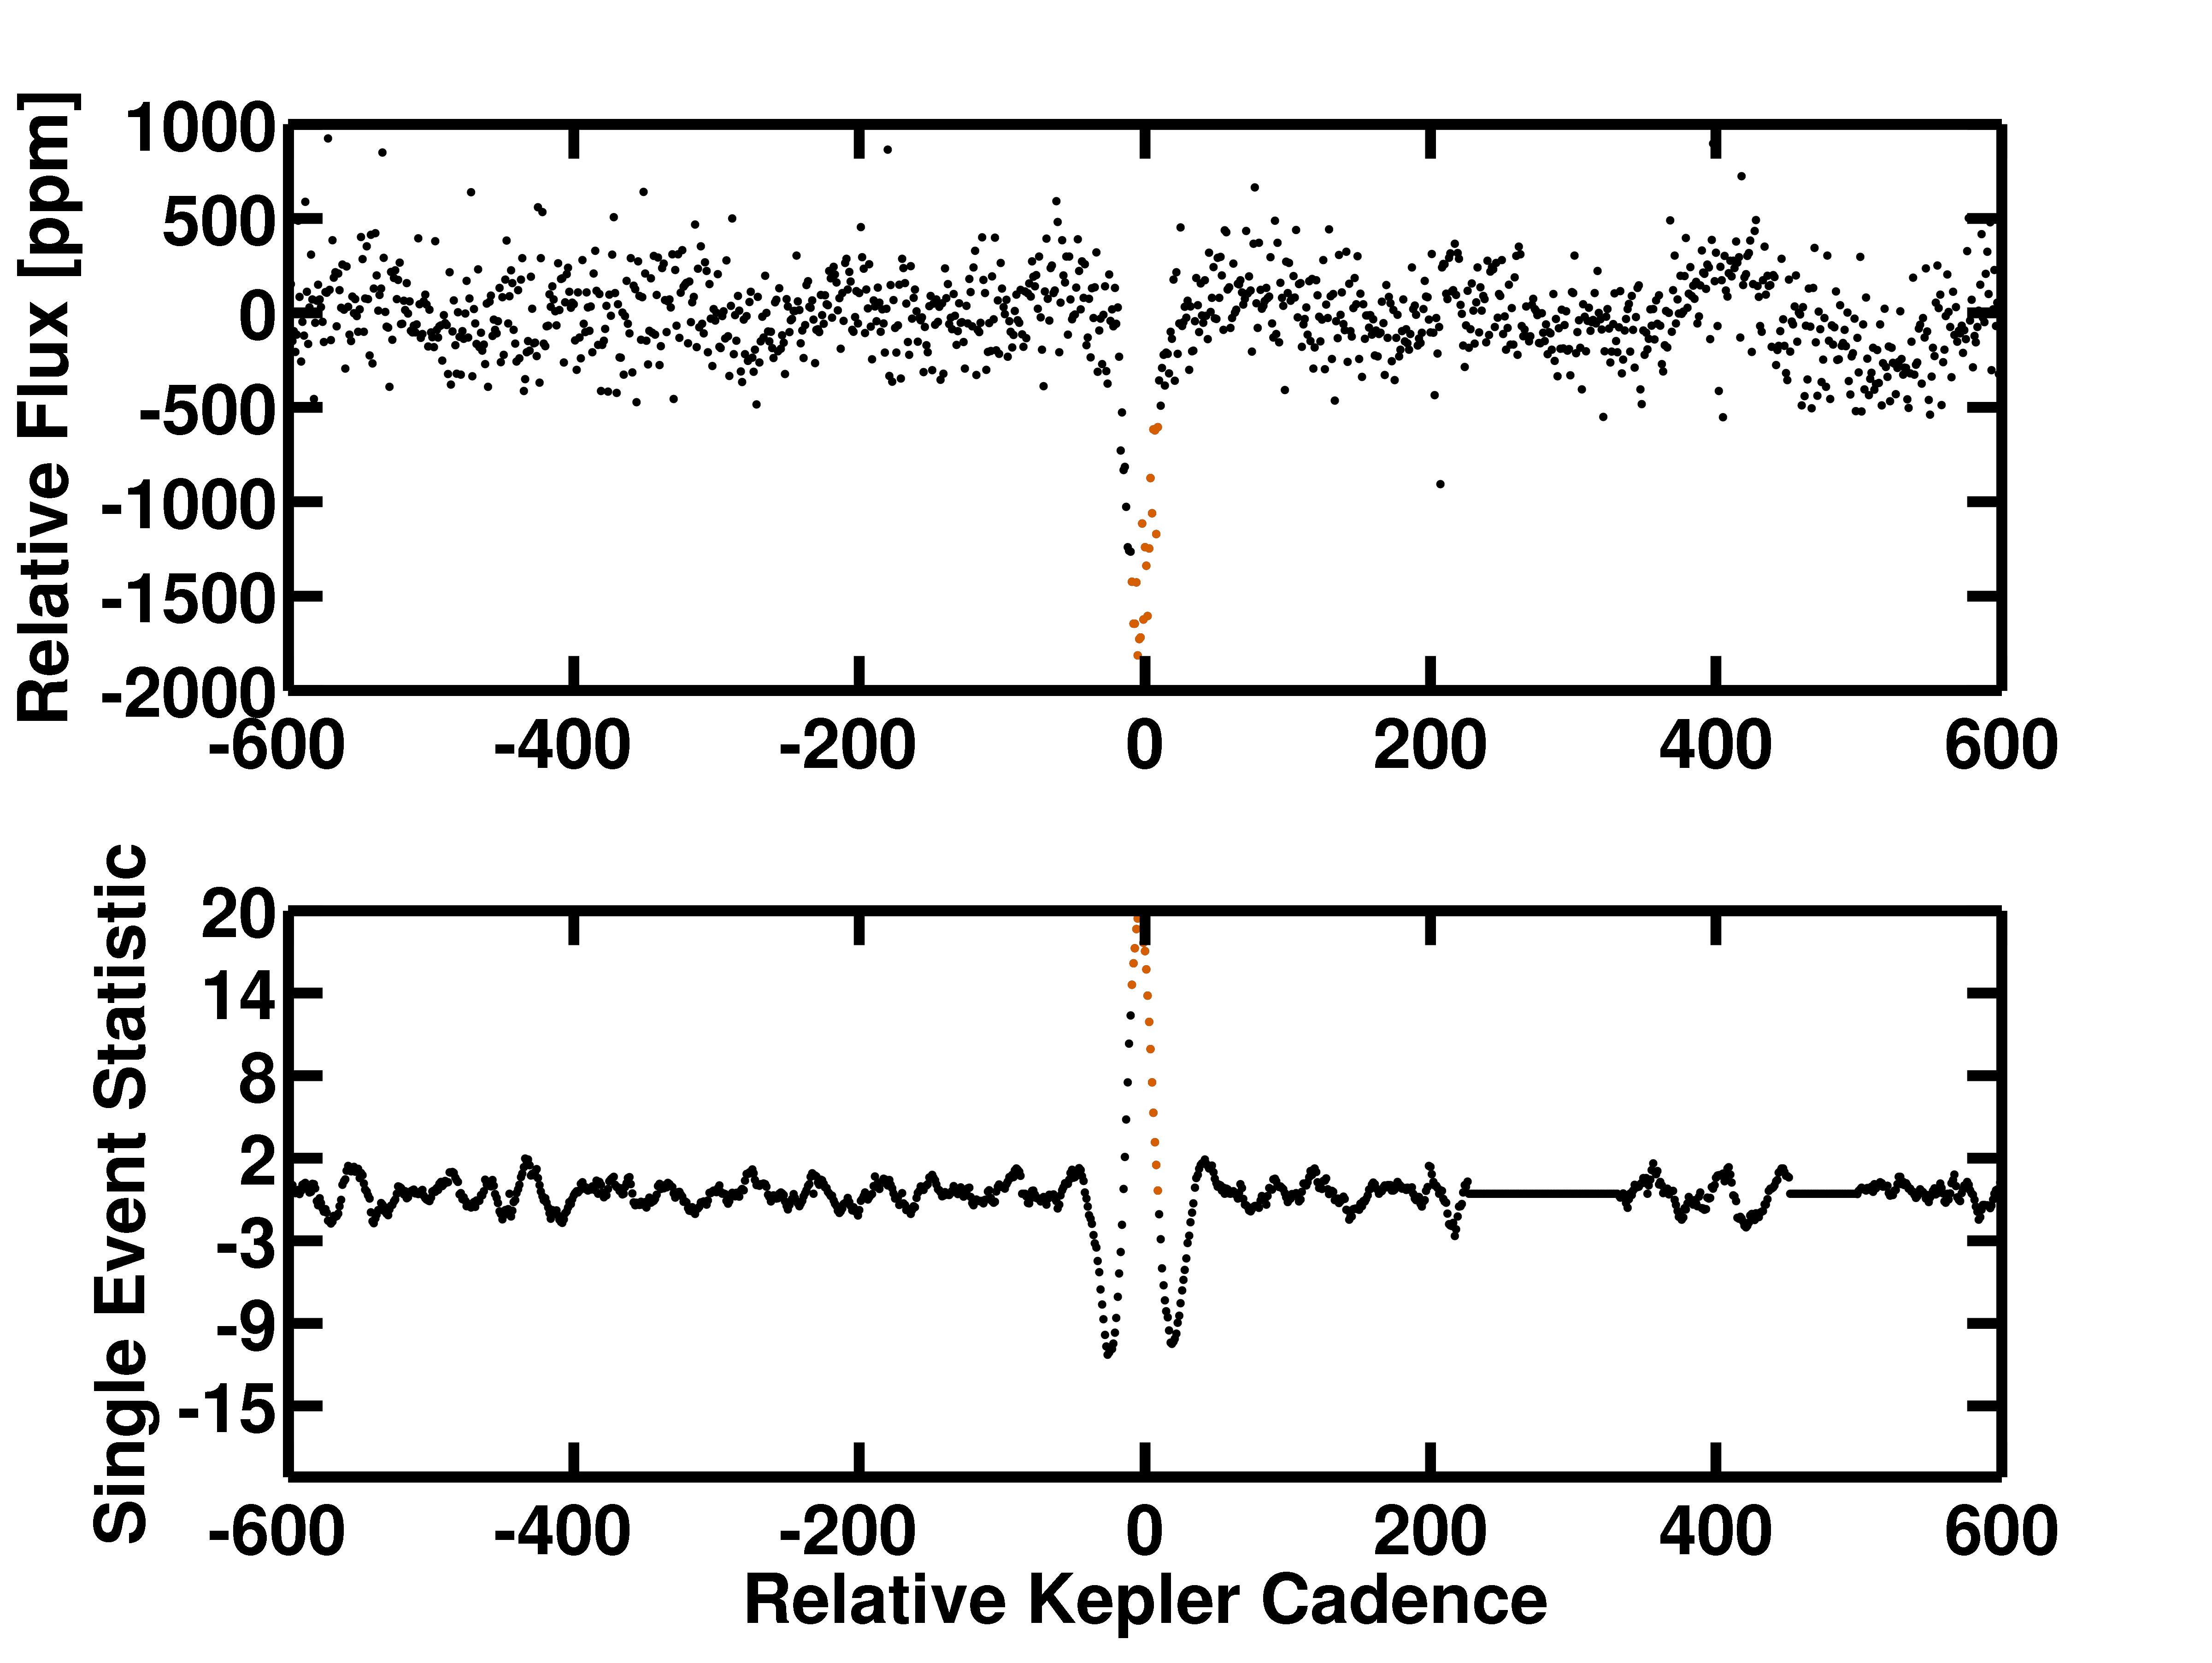
\includegraphics[width=0.5\textwidth]{kic11911580_cleanhighsnr.png}
\caption{Upper panel: flux time series for a single transit event contributing to the TCE for KOI 3900.01 on target KIC~11911580 (black points).  The cadences in transit (orange points) show a significant flux decrement relative to the baseline flux level.  Lower panel: SES time series of the transit event show in the upper panel, representing the archetypal shape of a transit signal displaying a strong central peak with two low-amplitude, symmetric side troughs. There are no other events as strong as the transit nearby in time so this signal has an individual transit event Chases metric, $Ch_{i}=1$.}
\label{fig:chases1}
\end{figure}

\begin{figure}[htb]
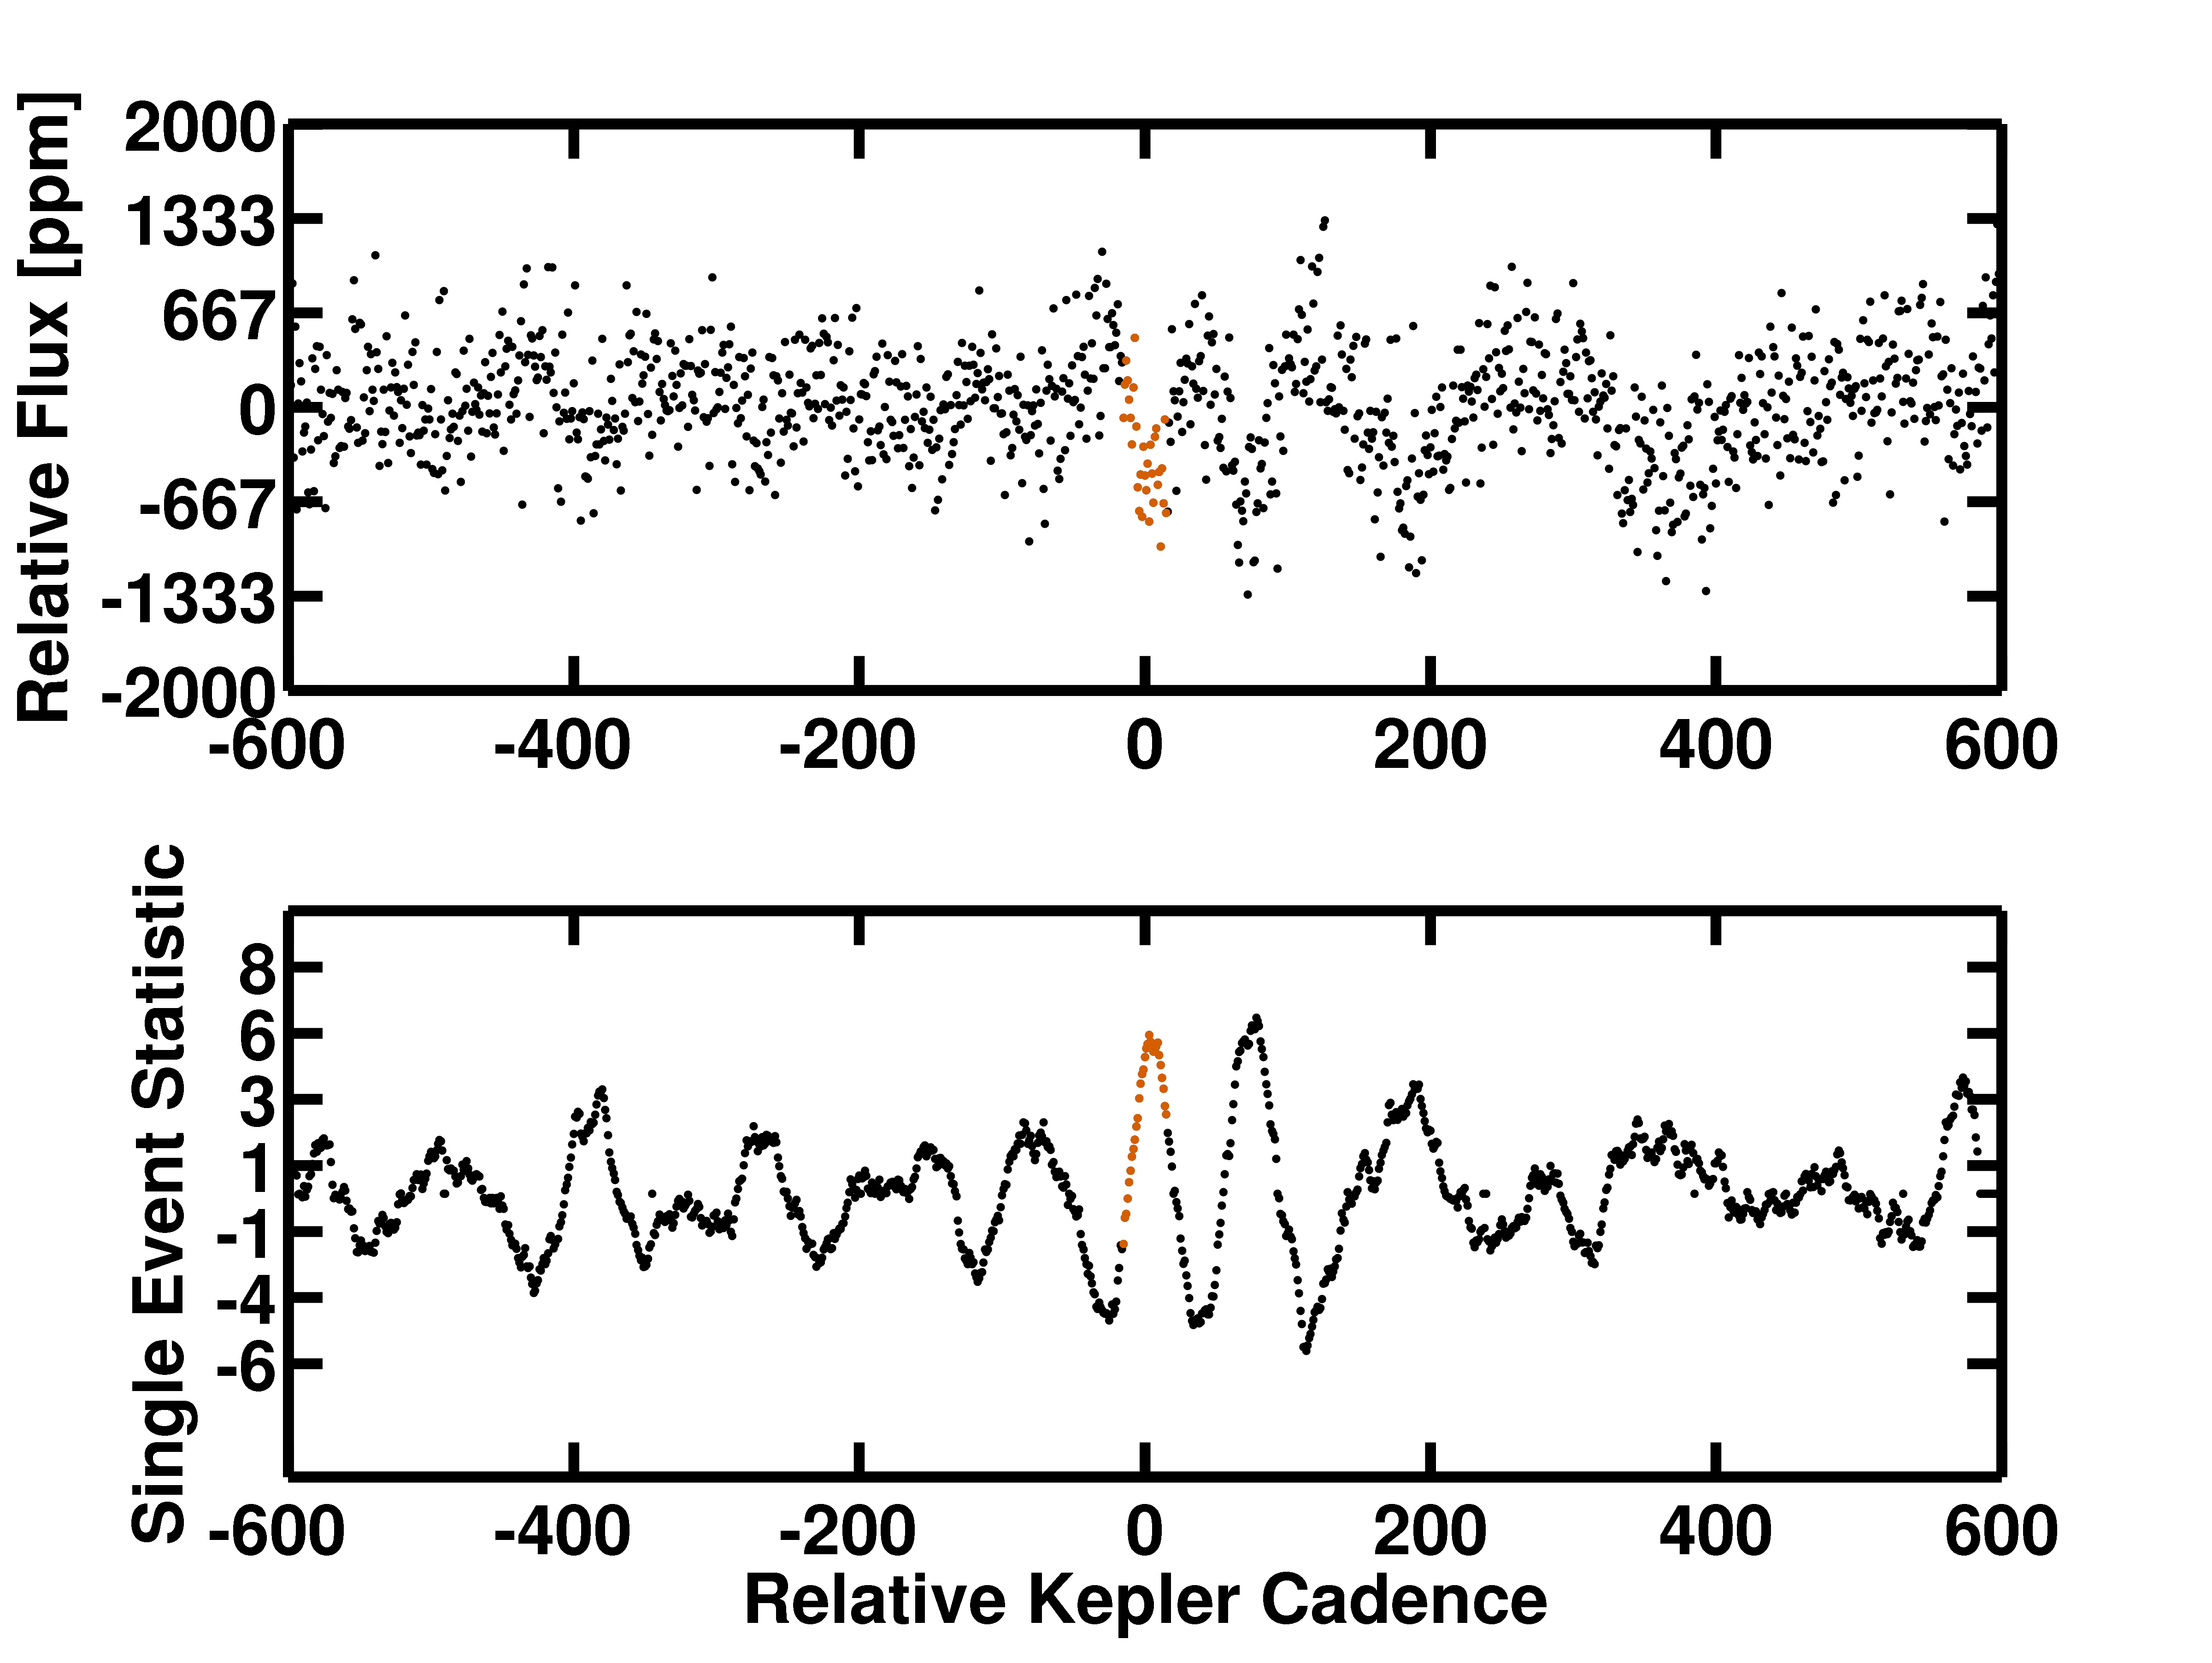
\includegraphics[width=0.5\textwidth]{kic11449918_rb.png}
\caption{Upper panel: flux time series for a single transit event contributing to the TCE on target KIC~11449918 (black points).  The cadences in transit (orange points) show a flux decrement, but there are numerous other flux decrements of similar depth and shape.  The instrumental ``rolling band'' pattern noise contributes systematics to the flux time series of target KIC 11449918 causing numerous signal detections.  Lower panel: SES time series of the transit event shown in the upper panel, representing the non-unique nature of the SES peak relative to surrounding data. The neighboring peak of comparable strength in the SES time series would result in $Ch_{i}=.016$ and the transit would be considered "bad" by Chases. }
\label{fig:chases2}
\end{figure}

\begin{figure}[htb]
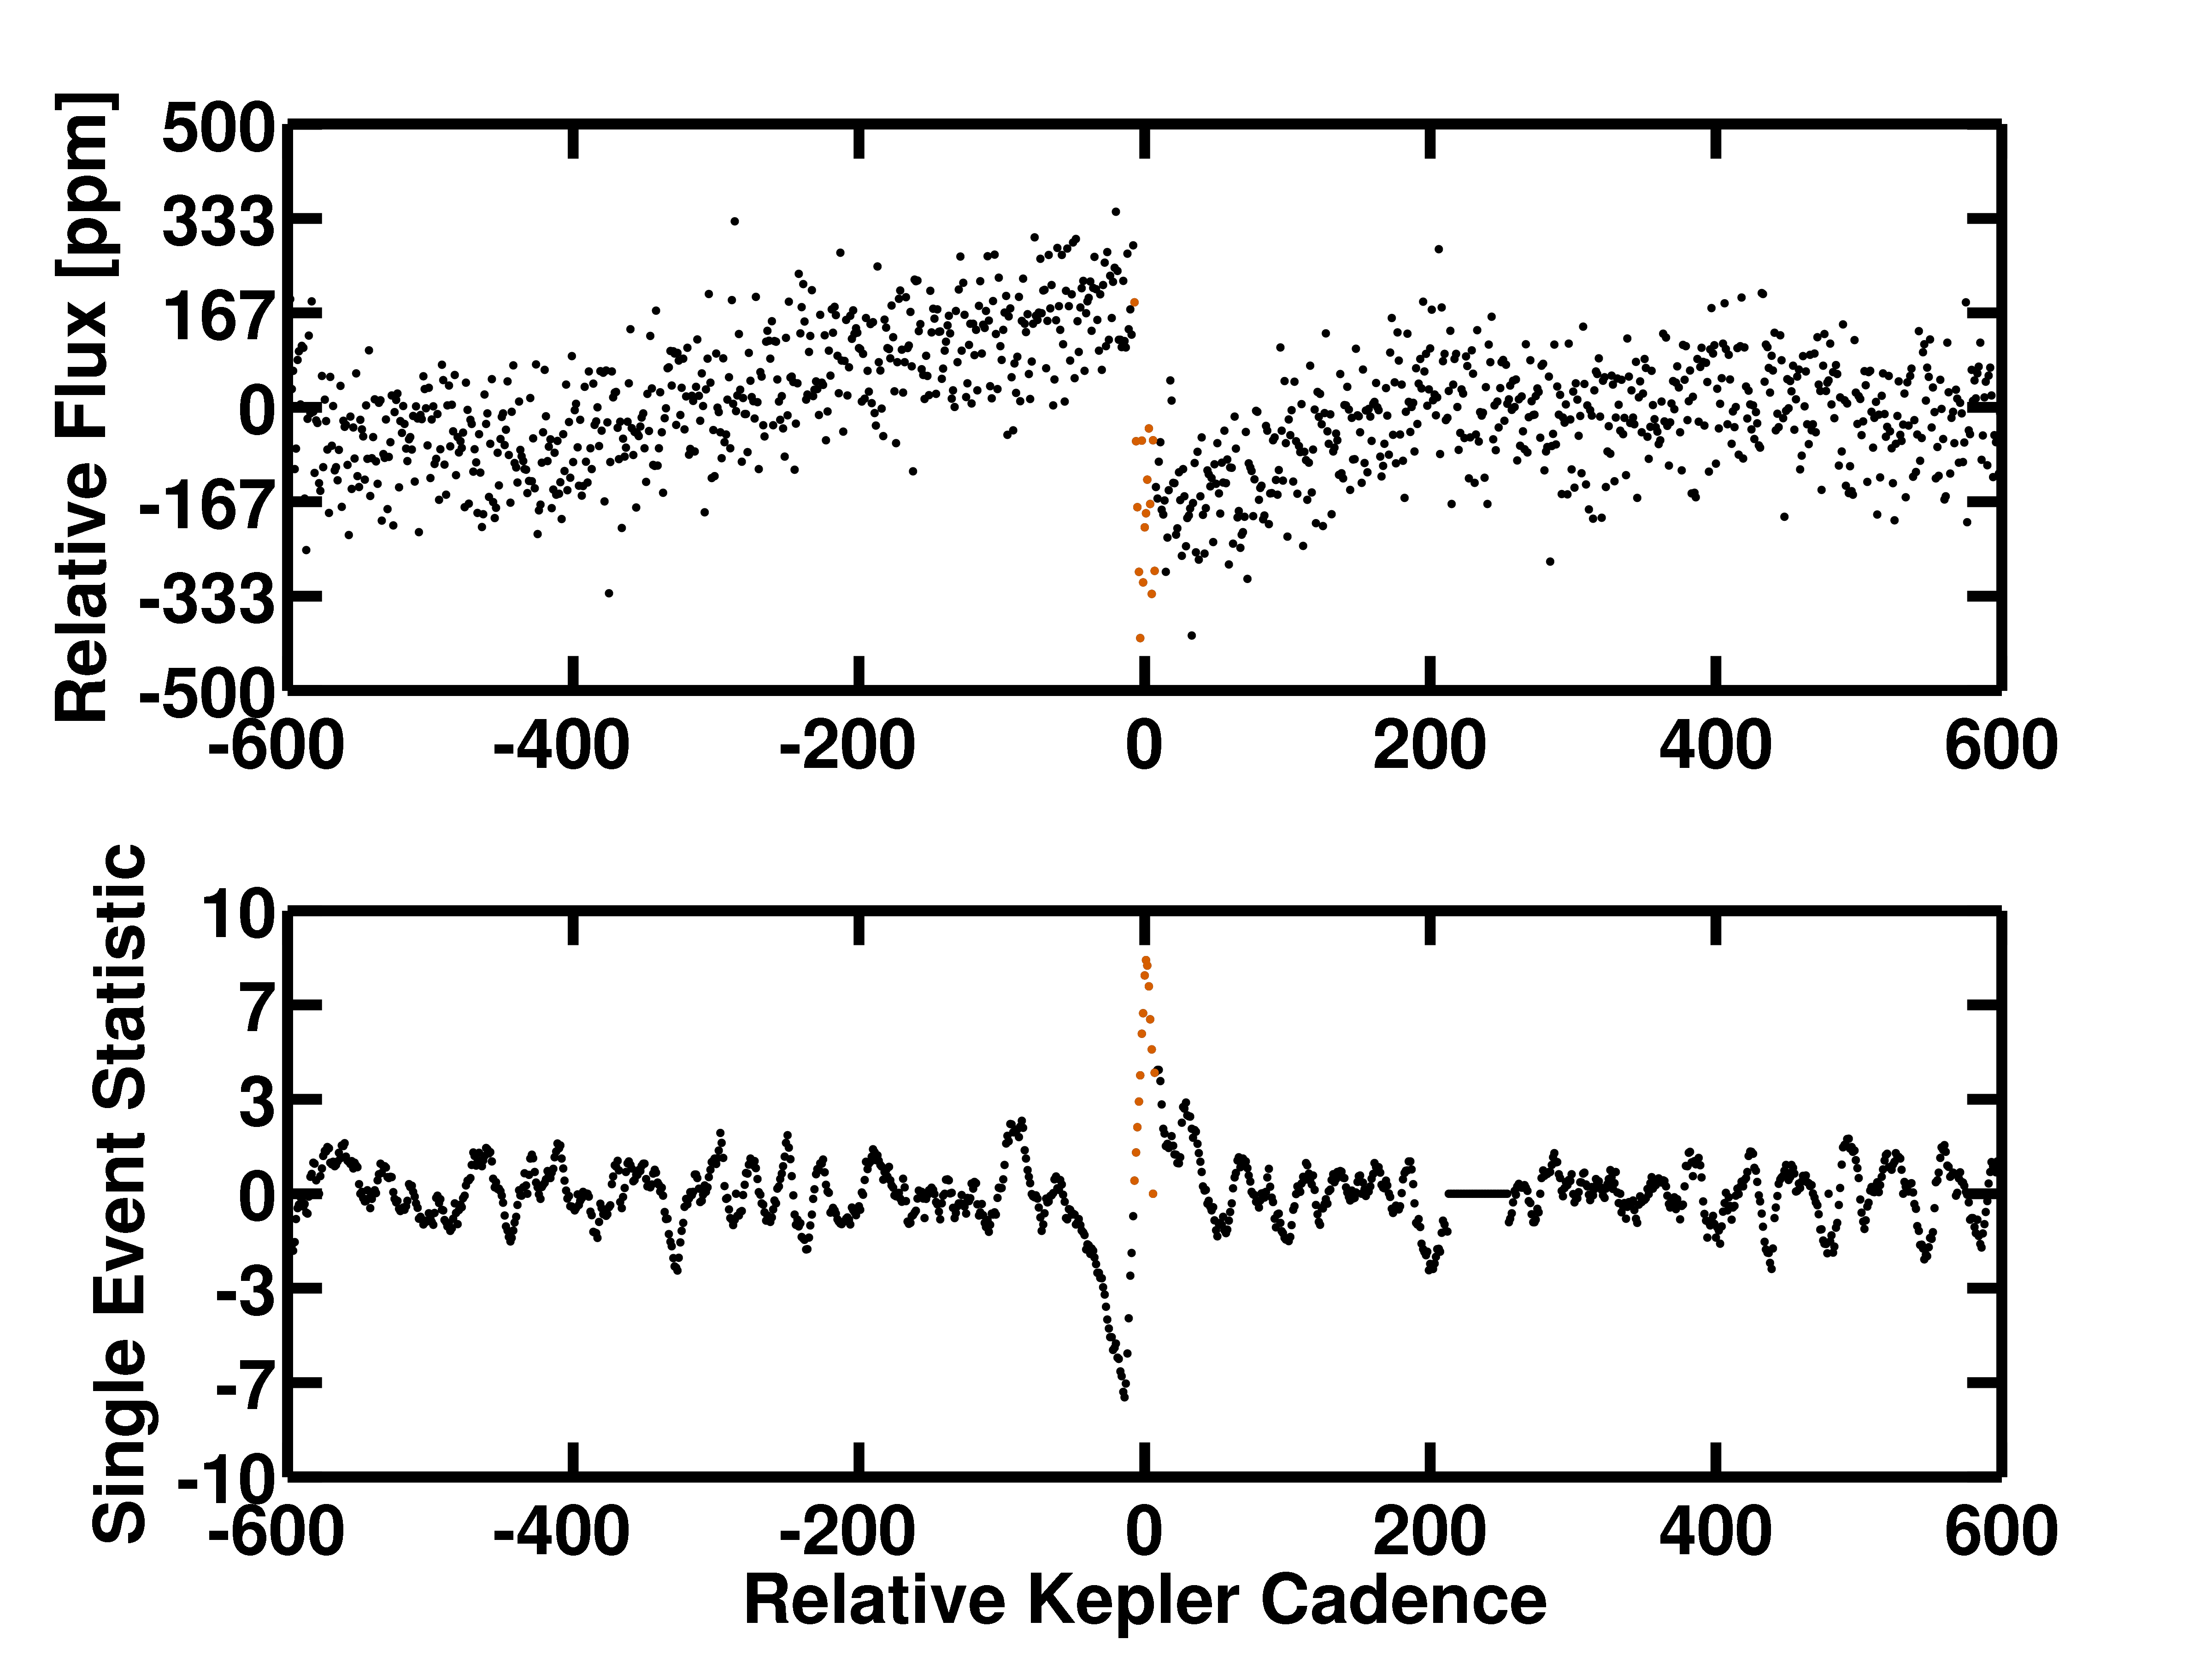
\includegraphics[width=0.5\textwidth]{kic12357074_spsd.png}
\caption{Upper panel: flux time series for a single transit event contributing to the TCE on target KIC 12357074 (black points).  The cadences in transit (orange points) show a flux decrement, but the sudden drop in flux followed by the gradual return to the baseline is archetypal of the SPSD instrumental signature.  Lower panel: SES time series for the transit event shown in the upper panel, illustrating the strongly asymmetric SES peak having a comparable amplitude negative SES trough preceding the SES peak. The neighboring trough of comparable absolute strength to the transit's peak would result in $Ch_{i}=.005$ and the transit would be considered "bad" by Chases.}
\label{fig:chases3}
\end{figure}


\paragraph{Skye -- Image Artifacts Clustered by Skygroup}
\label{s:skye}

As discussed in \ref{s:tces}, there are a number of TCEs caused by rolling-band image artifacts. These artifacts are caused by a spatial pattern in the CCD bias level that moves across the chip in response to changes in the temperature of the chip \citep[for more detail see ][]{VanCleve2009}. If a number of individual transit events from TCEs on different targets, but the same skygroup (region of the sky that falls on the same CCD each quarter), occur at the same time, they are very likely systematic in origin. The metric called Skye looks for an excess in the number of individual events occurring at the same time in the same skygroup. If an excess is identified we consider these events to be caused by artifacts. 

More specifically, for each skygroup we bin the individual events into 1.0\,d bins. We only use those \opstce\ with periods greater than 45\,d ($\sim$half a \Kepler\ quarter) for each skygroup. The reason for the period cut is that the long-period \opstce{s} are likely to be affected by rolling-band systematics, but the short-period ones are not.  Including shorter period TCEs would dramatically increase the number of individual transits and would reduce the significance of the anomalous peaks.  See Figure~\ref{skyefig} for an example of the anomalous peaks seen in some skygroups when the data is binned in this way.

To determine which events are anomalous, for each skygroup, we compute the average rate ($R$) of transits, by dividing the overall number of individual transit events in the skygroup by the number of 1.0\,d bins. Assuming the majority of transits are randomly distributed in time, and utilizing Poisson counting statistics, any peaks greater than:

\begin{equation}
\label{eq:skye}
\mathrm{threshold} = R + N*\sqrt{R}
\end{equation}

\noindent are statistically significant and indicative of temporal clustering, given a chosen value for $N$. We choose a value of $N = 3.0$, and robustly determine the rate for each skygroup by first computing the threshold using all the bins, then iteratively rejecting all bins with a height greater than threshold and re-computing threshold until it converges and does not change with further iterations.

For each skygroup and its threshold, we identify the individual times-of-transit for TCEs belonging to the skygroup that fall in bins that are above the threshold. We assign Skye a value of 1.0 to these individual transits to indicate they are bad transits. The Skye value for all other transit times are set to zero.

\begin{figure}[ht]
\centering
\begin{tabular}{c}
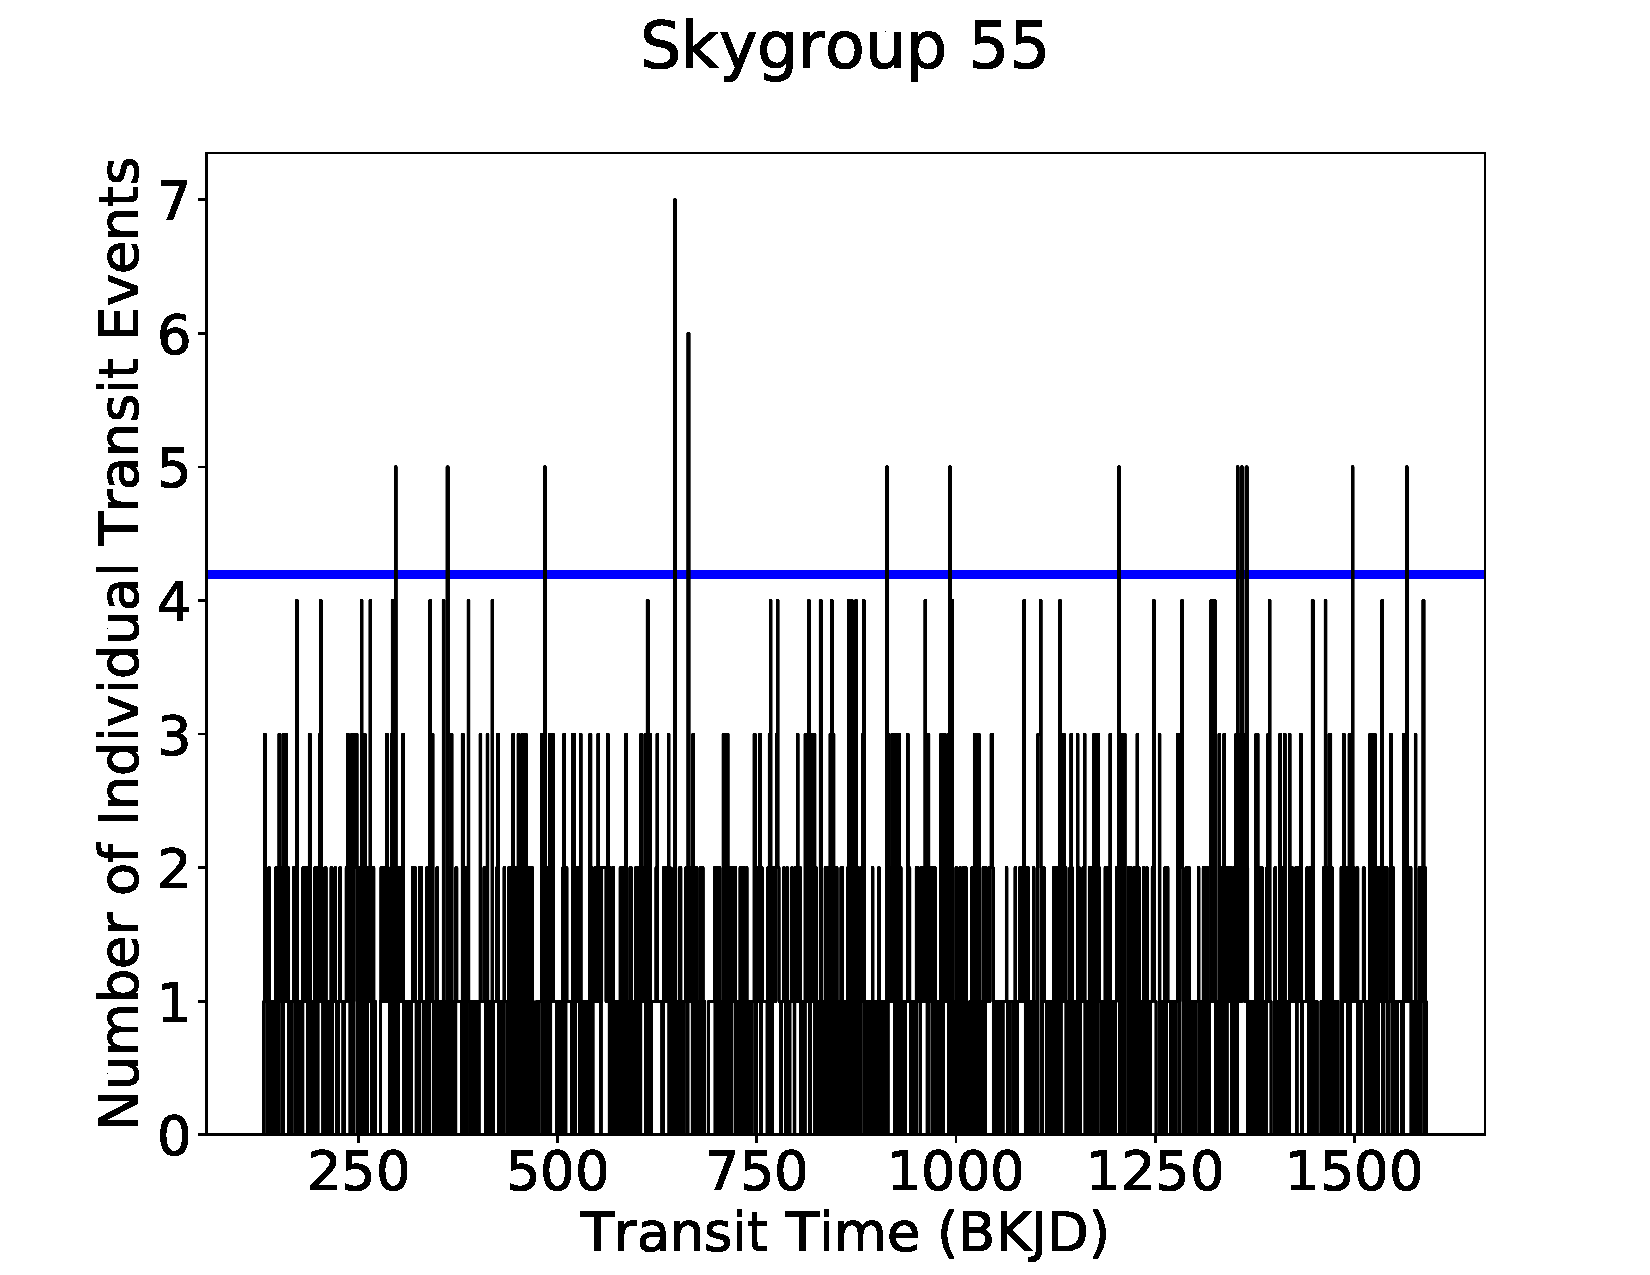
\includegraphics[width=\linewidth]{Skye-Paper-Plot-55.pdf}\\
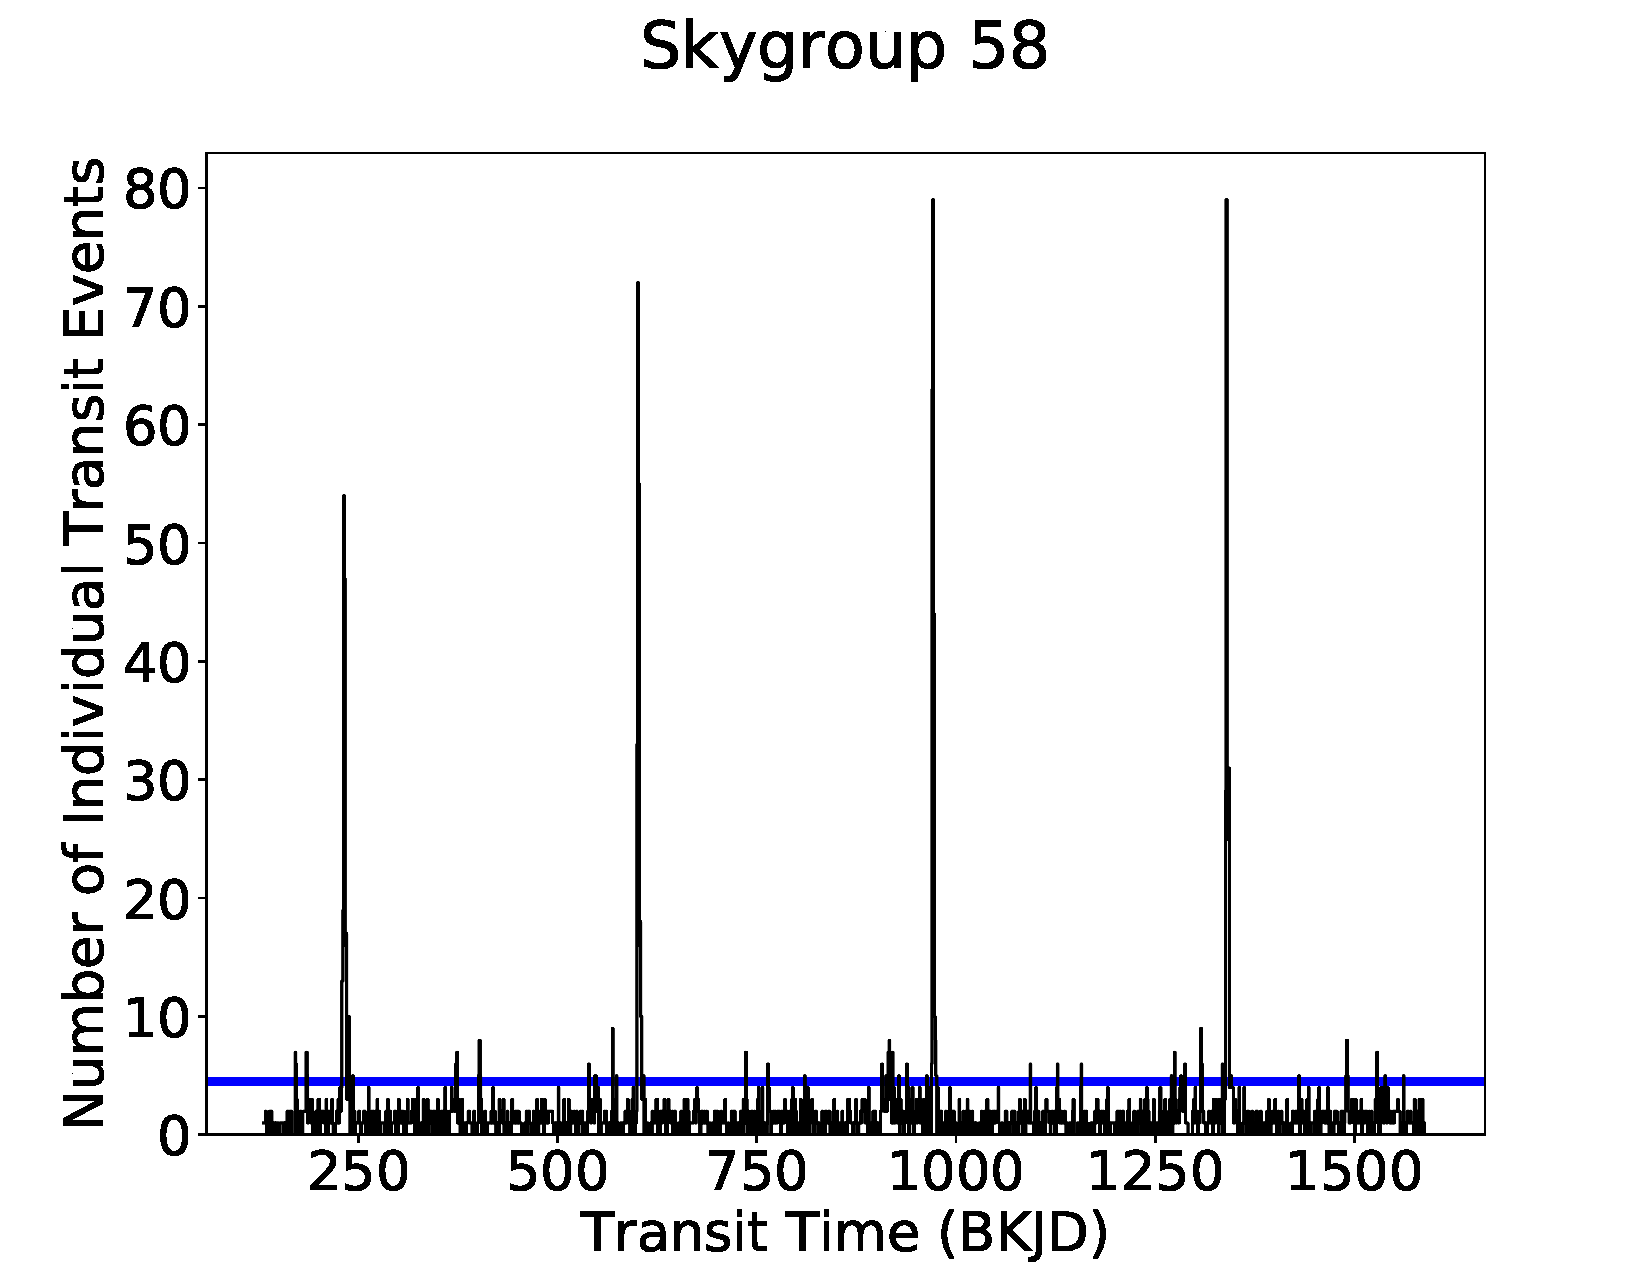
\includegraphics[width=\linewidth]{Skye-Paper-Plot-58.pdf}
\end{tabular}
\caption{An example of how the Skye metric flags individual transit events. The plots show the number of individual transit events (from TCEs with periods greater than 45 days) that occur in one-day time bins throughout the mission duration. Two of the 84 skygroups were chosen to be shown as examples, with skygroup 55 plotted on top, and skygroup 58 plotted on bottom. As can be seen, skygroup 58 has a strong clustering of transit events at times that correspond to the $\sim$372~day orbital period of the spacecraft, as the stars belonging to skygroup 58 fall on CCD channels with strong rolling-band signal. In contrast, skygroup 55 is nearly uniform. Individual transits that occur in a one-day time bin with a number of transit events above the threshold (shown by the blue horizontal line; see Equation~\ref{eq:skye}) are flagged as bad transits due to the Skye metric.}
\label{skyefig}
\end{figure}


\paragraph{Zuma -- Negative Significance}
\label{s:zuma}

A valid transit-like TCE should be comprised of individual events that correspond to flux decrements. If any event instead shows an increase of flux then that event is suspect. We thus designate any individual transit event with SES~$<$~0 as ``bad''.


\paragraph{Tracker -- Ephemeris Slip}
\label{s:tracker}
After the TPS module of the \kepler{} pipeline detects a TCE, it is sent to DV to be fit with a full transit model. DV allows the period and epoch to vary when fitting in order to provide as accurate a fit as possible. Sometimes the TPS ephemeris and DV ephemeris can end up significantly different. When this occurs it indicates that the underlying data is not transit-like and the TCE is likely due to quasi-sinusoidal systematics, which cause the ephemeris to wander when fitting.

Tracker measures (i.e. keeps track of) the time difference between the TPS and DV linear ephemerides in units of the TCE's duration for each transit. When Tracker is greater than  0.5 for any transit we designate the transit as bad.


% The metric formally known as Rocky
\subsubsection{Fraction of Gapped Events}
\label{s:rocky}

Due to the method of data gapping employed in TPS, sometimes the \kepler{} Pipeline can create a TCE that has a majority of its individual events occur where there is no actual in-transit data. This tends to happen particularly in multi-TCE systems, because once the \kepler{} Pipeline detects a TCE in a given system, it removes the data corresponding to the in-transit cadences of that TCE, and re-searches the light curve. 

We thus developed a metric that measures the number of individual transit events that actually contain data. Specifically, we compute the fraction of individual events with either SES~$\ne$~0 or Rubble~$>$~0.75, which indicate there is sufficient in-cadence data present. If the fraction of transits meeting these criteria is~$\le$~0.5, we fail the TCE as not transit-like.


\subsection{Stellar Eclipse}
\label{sigsecsec}

If a TCE is deemed transit-like by passing all of the tests presented in \S\ref{nottransitlikesec} on both detrendings, it is given a KOI number (see Figure~\ref{robovetter-transitlike-fig}).
However, many of these KOIs are FPs due to eclipsing binaries and contamination from nearby variable stars. We employ a series of robotic tests to detect systems that are due to stellar companions, as shown by the flowchart in Figure~\ref{robovetter-sigsec-fig}.

%In order to produce a uniform catalog, we do not designate any TCE an FP on the basis of its transit depth or inferred radius --- see \S7 item 6 of \citet{Mullally2015cat} for more detail. 

% us, being agnostic to stellar parameters, the only way to definitively detect an EB via a \kepler{} light curve is by detecting a significant secondary eclipse. 

%MENTION THE WHOLE FLAG SECONDARY -> STELLAR CHANGE, OR NOT? (Jeff translation: We used to call the S flag 'Significant Secondary' but now S is 'Stellar Eclipse', so do we want to explicitly mention that we made this change?)




\begin{figure*}[ht]
\centering
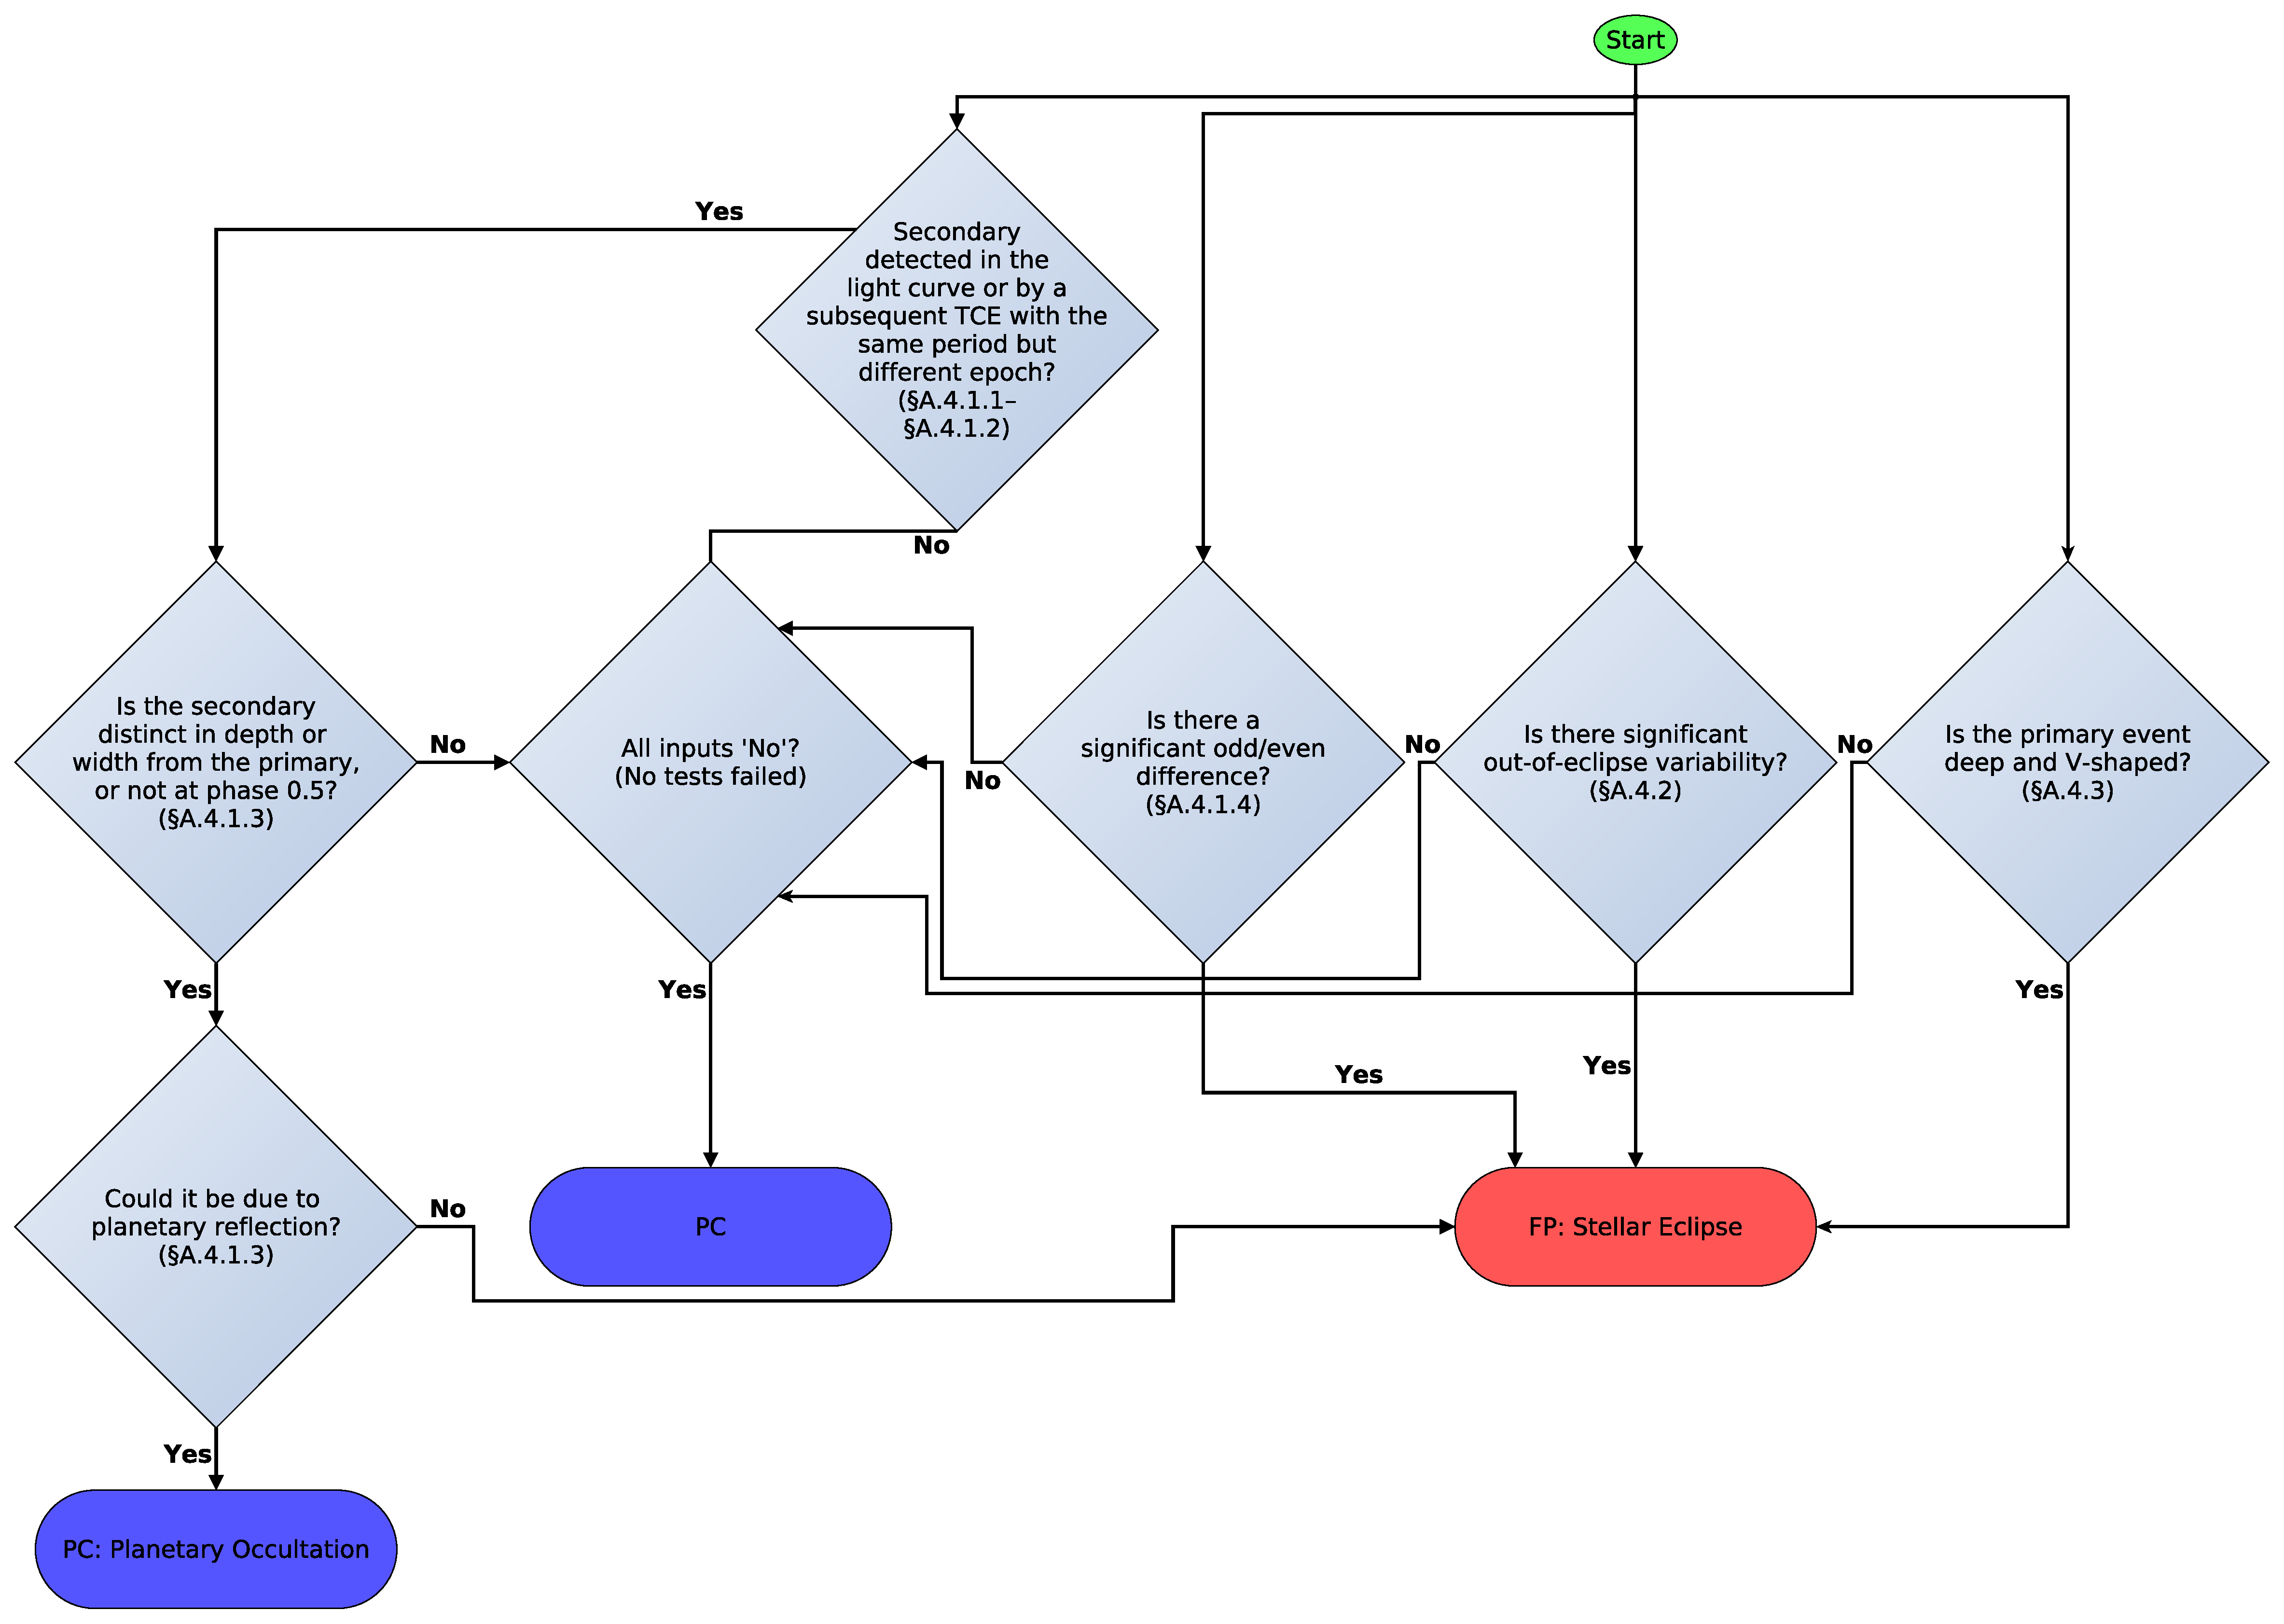
\includegraphics[width=\linewidth]{RoboVetter-Diagram-V4-SigSec.pdf}
\caption{Flowchart describing the stellar eclipse tests of the Robovetter. Diamonds represent ``yes'' or ``no'' decisions that are made with quantitative metrics. The multiple arrows originating from ``Start'' represent decisions that are made in parallel.}
\label{robovetter-sigsec-fig}
\end{figure*}


\subsubsection{Secondary Eclipse}

One of the most common methods to detect a stellar system is the presence of a significant secondary in the light curve. With the exception of some hot Jupiter type planets \citep[e.g., HAT-P-7,][]{Borucki2009}, the visibility of a secondary eclipse in \kepler{} data is a telltale sign of a stellar eclipsing binary.


\paragraph{Subsequent TCE With Same Period}
\label{s:secondTce}
Once the \kepler{} Pipeline detects a TCE in a given system, it removes the data corresponding to this event and re-searches the light curve. It is thus able to detect the secondary eclipse of an eclipsing binary as a subsequent TCE, which will have the same period, but different epoch, as the primary TCE. Thus, utilizing equations~\ref{peq1}-\ref{peq3}, the Robovetter dispositions a TCE as a stellar system FP if its period matches a subsequent TCE within the utilized tolerance ($\sigma_{P}$ $>$ 3.25) and they are separated in phase by at least 2.5 times the transit duration. For clarity, we note again that it is sometimes possible that the periods of two TCEs will meet the period matching criteria, but be different enough to have their epochs shift significantly in phase over the $\sim$4 year mission duration. The phase separation requirement must be upheld over the entire mission duration in order to disposition the TCE as an FP due to a significant secondary.  

Occasionally the \kepler{} Pipeline will detect the secondary eclipse of an eclipsing binary at half, third, or some smaller integer fraction of the orbital period of the system. In these cases, the epoch of the TCE corresponding to the secondary will overlap with that of the primary. These cases are accounted for by not requiring a phase separation of at least 2.5 transit durations when a period ratio other than unity is detected. (Note that equations~\ref{peq1}-\ref{peq3} allow for integer period ratios.) While this approach will likely classify any multi-planet system in an exact 2:1 orbital resonance as an FP due to a significant secondary, in practice this is non-existent. Exact 2:1 orbital resonances, where ``exact'' means the period ratio is close enough to 2.0 over the $\sim$4 year mission duration to avoid any drift in relative epoch, appear to be extremely rare \citep{Fabrycky2014}. Also, they might produce strong transit timing variations, which would likely preclude their detection. The \kepler{} pipeline employs a strictly linear ephemeris when searching for TCEs, and thus while planets with mild transit timing variations (TTVs), e.g., deviations from a linear ephemeris less than the transit duration, are often detected, planets with strong TTVs, e.g., deviations from a linear ephemeris greater than the transit duration, are often not detected.



\paragraph{Secondary Detected in Light Curve}
\label{secdetectsec}
\label{s:second}

There are many cases when a secondary eclipse does not produce its own TCE, most often when its MES is below the \kepler{} Pipeline detection threshold of 7.1. The model-shift uniqueness test, discussed in \S\ref{s:ms}, is well-suited to automatically detect secondary eclipses in the phased light curve, as it searches for the next two deepest events aside from the primary event. It is thus able to detect the best-candidate secondary eclipse in the light curve and assess its significance. We compute the following quantities to use as secondary detection metrics

\begin{equation}
    MS_{4} = \sigma_{\rm Sec}/F_{\rm Red} - FA_{1}
\end{equation}

\begin{equation}
    MS_{5} = (\sigma_{\rm Sec} - \sigma_{\rm Ter}) - FA_{2}
\end{equation}

\begin{equation}
    MS_{6} = (\sigma_{\rm Sec} - \sigma_{\rm Pos}) - FA_{2}
\end{equation}

Recall that $\sigma$ indicates a significance and was defined in \S\ref{s:ms}. If $MS_{4}$~$>$1, $MS_{5}$~$>$0, and $MS_{6}$~$>$0, in either the DV or alternate detrendings, the Robovetter dispositions the TCE as a stellar system FP. These criteria ensure that the secondary event is statistically significant when compared to the systematic noise level of the light curve, the tertiary event, and the positive event, respectively.

\paragraph{Candidates with Significant Secondaries}
\label{s:sscand}
There are two exceptions when the above-mentioned conditions are met, but the Robovetter does not designate the TCE as an FP. First, if the primary and secondary widths and depths are statistically indistinguishable, and the secondary is located at phase 0.5, then it is possible that the TCE is a PC that has been detected at twice the true orbital period. Thus, the Robovetter labels a TCE with a significant secondary as a PC when ${\sigma_{\rm Pri} - \sigma_{\rm Sec} < FA_{2}}$ and the phase of the secondary is within 1/4 of the primary transit's duration of phase 0.5. Second, hot Jupiter PCs can have detectable secondary eclipses due to planetary occultations via reflected light and thermal emission \citep{Coughlin2012}. Thus, a TCE with a detected significant secondary is labeled as a PC with the significant secondary flag (in order to facilitate the identification of hot Jupiter occultations) when the geometric albedo is less than 1.0, the planetary radius is less than 30~\re{}, the depth of the secondary is less than 10\% of the primary, and the impact parameter is less than 0.95. The additional criteria beyond the albedo criterion are needed to ensure that this test is only applied to potentially valid planets and not grazing eclipsing binaries. We calculate the geometric albedo by using the stellar mass, radius, and effective temperature from the DR25 stellar catalog \citep{Mathur2017ApJS}, and the values of the period and radius ratio from the original DV fits.



\paragraph{Odd/Even Depth Difference}

\label{s:oddeven}
If the primary and secondary eclipses of eclipsing binaries are similar in depth, and the secondary is located near phase 0.5, the \kepler{} pipeline may detect them as a single TCE at half the true orbital period of the eclipsing binary. In these cases, if the primary and secondary depths are dissimilar enough, it is possible to detect it as an FP by comparing the depths of the odd- and even-numbered transit events and their associated uncertainties, via the following statistic:

\begin{equation}
\sigma_{\rm OE} = \frac{abs\left(d_{\rm odd} - d_{\rm even}\right)}{\sqrt{\sigma_{odd}^{2} + \sigma_{even}^{2}}} ,
\end{equation}

\noindent where $d_{\rm odd}$ is the measured depth using the odd-numbered transits, with associated uncertainty $\sigma_{odd}$, $d_{\rm even}$ is the measured depth using the even-numbered transits, with associated uncertainty $\sigma_{even}$, and abs() returns the absolute value.

We use two different methods to compute $d_{\rm odd}$, $\sigma_{odd}$, $d_{\rm even}$, $\sigma_{even}$, and thus $\sigma_{\rm OE}$, for both for the DV and alternate detrending. For the first method, the depths are computed by taking the median of all the points near the center of all transits, and the uncertainty is the standard deviation of those points, both using only the odd- or even-numbered transits. For the alternate detrending with a trapezoidal fit, we use all points that lie within $\pm$30 minutes of the central time of transit, as well as any other points within the in-transit flat portion of the trapezoidal fit. For the DV detrending, we use all points within $\pm$30 minutes of the central time of transit. (This threshold corresponds to the long-cadence integration time of the \kepler{} spacecraft. Including points farther away from the central time of transit degrades the accuracy and precision of the test.) If $\sigma_{\rm OE}$ $>$ 1.1 for either the DV or alternate detrending then the TCE is labeled as an FP due to a significant secondary and given the DEPTH\_ODDEVEN\_DV and/or DEPTH\_ODDEVEN\_ALT flag(s). The value of 1.1 was empirically derived utilizing manual checks and transit injection. This method is very robust to outliers and systematics, but not extremely sensitive as it does not take into account the full transit shape to measure the depth.

The second method measures the depths and uncertainties by running the Modelshift test separately on the portions of the light curve within half a phase of the odd- and even-numbered transits. Modelshift measures the depths and associated uncertainties by utilizing the entire transit model and taking into account the measured noise level of the entire light curve. This method is more sensitive to small odd/even differences, but also more sensitive to outliers and light curve systematics compared to the above method. If $\sigma_{\rm OE}$ $>$ 11.2 for the DV detrneidng, or $>$ 19.8 for the alternate detrending, then the TCE is labeled as an FP due to a significant secondary and given the MOD\_ODDEVEN\_DV and/or MOD\_ODDEVEN\_ALT flag(s). The thresholds of 11.2 and 19.8 were empirically derived utilizing manual checks and transit injection. This method is susceptible to outliers and systematics (and why the thresholds are set fairly high), but can also detect small, yet significant odd/even differences that the other method listed above cannot.


\subsubsection{Out of Eclipse Variability}
\label{s:sweeteb}
Short-period eclipsing binaries will often show out-of-eclipse variability due to tidal forces that deform the star from a perfect spheroid. The variability manifests as quasi-sinusoidal variations at either the period, or half the period, of the binary.

We use the information from SWEET (see~\S\ref{s:sweetntl}) to detect these cases. If a transit-like TCE has a SWEET SNR greater than 50, an amplitude less than the TCE transit depth in either the DV and ALT detrendings, an amplitude greater than 5,000~ppm, and a period less than 10 days, we fail it as a stellar system.



\subsubsection{V-Shape Metric}
\label{s:shapemetric}
There are cases of eclipsing binaries that do not show a secondary eclipse, either due to the secondary star being too low luminosity for the eclipse to be detectable, or the binary has significant eccentricity and a longitude of periastron such that geometrically no eclipse occurs. Also, most detached eclipsing binaries will not exhibit detectable out-of-eclipse variability. In these cases, the only remaining way to infer that the signal is due to a stellar system and not a planet is to utilize the shape and depth of the transit.

In previous catalogs \citep{Rowe2015cat,Mullally2015cat,Coughlin2016} TCEs were not failed based on their inferred radii alone. This was on purpose as the catalogs attempted to be as agnostic to stellar parameters as possible, such that dispositions would remain applicable if and when better stellar parameters were obtained, e.g., by GAIA \citep{Cacciari2009,Mignard2005}. This resulted in some PC KOIs with large depths that were known to very likely be eclipsing binaries, and in fact were later confirmed as such by follow-up observations \citep{Santerne2016}.

In this catalog, we attempt to strike a balance between identifying these binary systems, while still remaining agnostic to stellar parameters. We adapted a simple shape parameter, originally used in \citet{Batalha2013}, and express it as the sum of the modeled radius ratio and the impact parameter. This metric reliably identifies eclipsing binaries both due to being too deep (large $R_{p}$/$R_{\star}$) and due to grazing eclipses (large impact parameter, $b$). Specifically we fail a transit-like TCE as a stellar system if $R_{p}$/$R_{\star}$~+~$b$~$>$~1.04.



\subsection{Centroid Offset}
\subsubsection{Centroid Robovetter}
\label{s:centroidrv}
The Robovetter relies on a piece of code called the Centroid Robovetter \footnote{\url{https://sourceforge.net/projects/keplercentroidrobovetter/}}\citep{Mullally2017} to detect when a transit signal originates from a background or nearby star instead of from the target star. The Centroid Robovetter has not changed since its implementation for the DR24 KOI catalog; we summarize it below for completeness. 

Given that \kepler 's pixels are 3.98\arcsec{} square \citep{Koch2010}, and the typical photometric aperture has a radius of 4--7 pixels \citep{Bryson2010b}, it is quite common for a given target star to be contaminated by light from another star. If that other star is variable, then that variability will be visible in the target aperture at a reduced amplitude. If the variability due to contamination results in a TCE, then it is a false positive, whether the contaminator is an eclipsing binary, planet, or other type of variable star \citep{Bryson2013}. For example, if a transit or an eclipse occurs on a bright star, a shallower event may be observed on a nearby, fainter star. Similarly, a star can be mistakenly identified as experiencing a shallow transit if a deep eclipse occurs on a fainter, nearby source.

The DV module of the \kepler{} Pipeline produces difference images for each quarter, which are made by subtracting the average flux in each pixel during each transit from the flux in each pixel just before, and after, each transit \citep{Bryson2013}. If the resulting difference image shows significant flux at a location (centroid) other than the target, then the TCE is likely an FP due to a centroid offset.

In our robotic procedure to detect FPs due to centroid offsets, we first check that the difference image for each quarter contains a discernible stellar image and is not dominated by background noise. This is done by searching for at least 3 pixels that are adjacent to each other and brighter than a given threshold, which is set by the noise properties of the image. We use an iterative sigma clipping approach to eliminate bright pixels when calculating the background noise, as the star often dominates the flux budget of a substantial number of pixels in the aperture.

For the difference images that are determined to contain a discernible stellar image, we first search for evidence of contamination from sources that are resolved from the target. Since resolved sources near the edge of the image may not be fully captured, Pixel Response Function (PRF --- \keplers{} point spread function convolved with the image motion and the intra-pixel CCD sensitivity) fitting approaches do not often work well to detect them. Instead, we check if the location of the brightest pixel in the difference image is more than 1.5 pixels from the location of the target star. If at least two-thirds of the quarterly difference images show evidence of an offset by this criterion, we disposition the TCE as an FP due to a centroid offset. % Note that FPs due to stars located many pixels from the target, i.e., far outside the target's image, are not detected by this approach, but rather through ephemeris matching (see \S\ref{ephemmatchsec}).

If no centroid offset is identified by the previous method, we then look for contamination from sources that are unresolved from the target. We measure the PRF-fit centroid of the difference images and search for statistically significant shifts with respect to the PRF centroid of both the out-of-transit images, as well as the catalog position of the source. Following \citet{Bryson2013}, a TCE is marked as an FP due to a centroid offset if there are at least three difference images with a discernible stellar image, and a 3$\sigma$ significant offset larger than 2$\arcsec$, or a 4$\sigma$ offset larger than 1$\arcsec$ is measured.  
%If any of these are not true, a flag is set indicating that fact.

The Centroid Robovetter gives the \kepler\ Robovetter several flags to indicate whether a centroid offset was detected and whether that detection can be trusted. The names of those flags have been changed for DR25 to be consistent with our minor flag naming scheme. A list of the minor flags are available in Appendix~\ref{s:minorflags}.


\subsubsection{Ghost Diagnostic}
\label{s:ghost}
The last method we use to detect a centroid offset is the ghost diagnostic, which was added to the DR25 \kepler{} Pipeline \citep[see \S\,11.3.7 of][]{JenkinsKDPH}. It determines whether a transit signal is likely contamination from a ghost image of a star located away from the target star in the focal plane. Ghost reflections occur when light from a bright star is reflected off the CCD and again from the field flattener plate and back onto the CCD. It appears as a diffuse, out-of-focus image of the pupil of the telescope. A similar type of false positive results from direct PRF (Pixel Response Function) contamination, when flux from the broad wings of a bright star near the target star on the CCD overlaps the target star's PRF.  If a ghost reflection (or the PRF of a nearby star) containing a transit-like signature (e.g. an eclipsing binary signal) overlaps the PRF of the target star, then the contaminating transit signal will be equally strong in the periphery and the core of the target. 

To detect this type of false alarm, the ghost diagnostic essentially measures the strength of the TCE signal in two separate light curves --- one created using the average of the pixels inside the target's optimal aperture minus the average of the pixels in an annulus surrounding the target aperture (core aperture correlation statistic), and the other using the average of the pixels in the annulus surrounding the target aperture (halo aperture correlation statistic). If the ratio of the halo aperture to core aperture statistic is greater than 4.0, the TCE is marked as an FP with the major flag set to Centroid Offset. This ghost diagnostic is not available to vet the \scrtce{s} and thus the reliability measured with that set of TCEs will be too small by an insignificant amount.



\subsection{Ephemeris Matching}
\label{ephemmatchsec}
\label{s:ephemmatch}

Another method for detecting FPs due to contamination is to compare the ephemerides (periods and epochs) of TCEs to each other, as well as other known variable sources in the \kepler{} field. If two targets have the same ephemeris within a specified tolerance, then at least one of them is an FP due to contamination. \citet{Coughlin2014a} used Q1--Q12 data to compare the ephemerides of KOIs to each other and eclipsing binaries known from both \kepler{}- and ground-based observations. They identified over 600 FPs via ephemeris matching, of which over 100 were not known as FPs via other methods. They also identified four main mechanisms of contamination. The results of \citet{Coughlin2014a} were incorporated in \citet[][see \S3.3]{Rowe2015a}. \citet[][see \S5.3]{Mullally2015cat} slightly modified the ephemeris matching process of \citet{Coughlin2014a}, and applied it to all of the Q1--Q16 TCEs, as well as known KOIs and eclipsing binaries, identifying nearly 1,000 TCEs as FPs. The same process was again used in the \citet{Coughlin2016} catalog.

We modify the matching criteria used in previous catalogs to obtain more accurate matches, due especially to the very large number of long-period TCEs encountered in DR25 compared to previous activities. We utilize the results of the transit injection run (\S\ref{s:simulated}) to measure the ability of the original DV fits by the \kepler{} Pipeline to recover period and epoch as a function of period. In Figure~\ref{injephemfig} we show, in the top two panels, the difference in the injected and recovered period and epoch, as a function of the injected period. The bottom panels show the measured standard deviation of the difference as a function of period, in linear and logarithmic space respectively. The red line is the result of a best-fit power law.

\begin{figure*}[ht]
\centering
\begin{tabular}{cc}
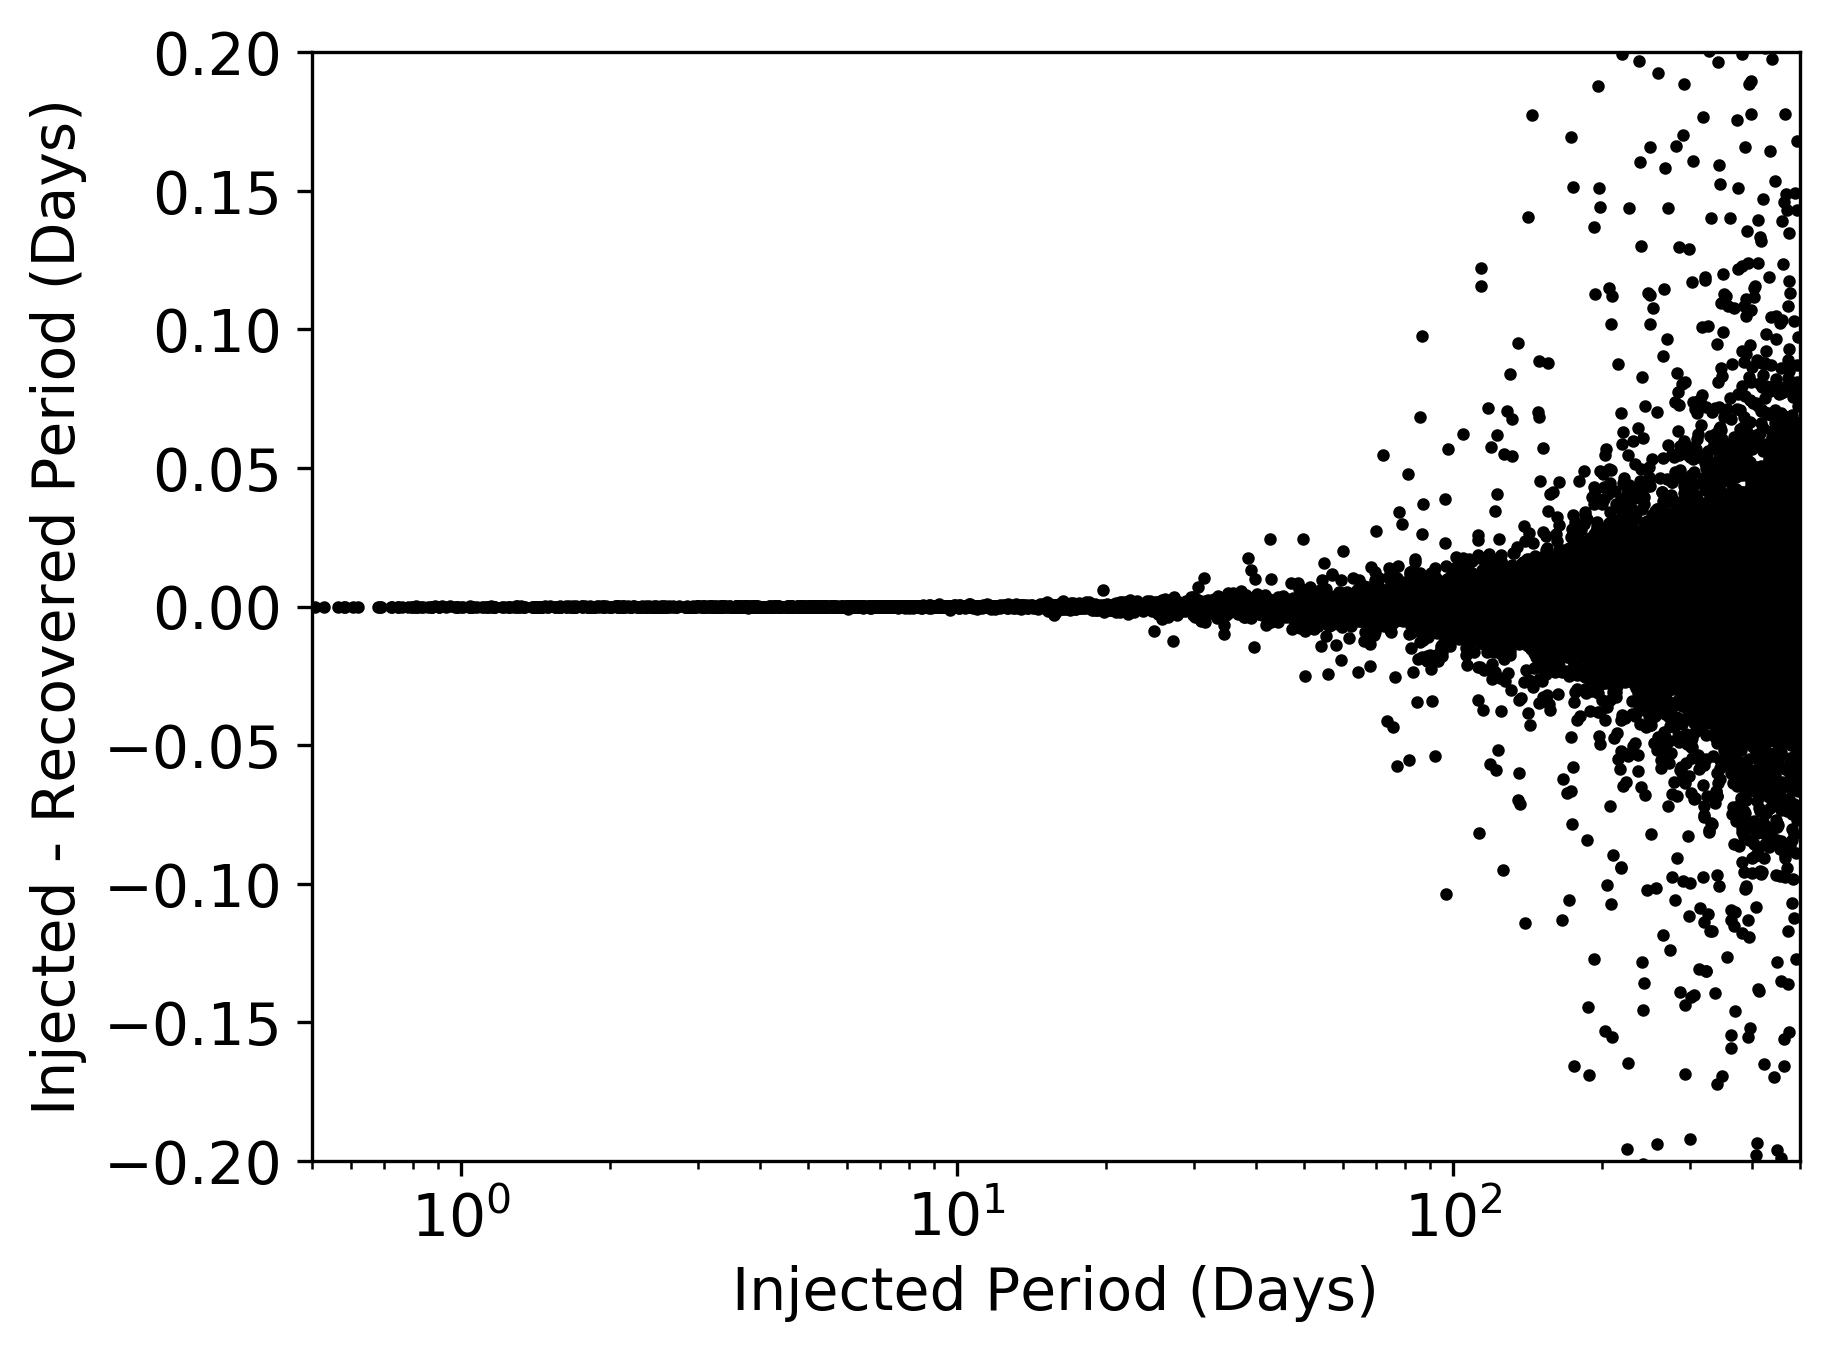
\includegraphics[width=0.5\linewidth]{INJ1-Ephem-Recovery-1.png} &
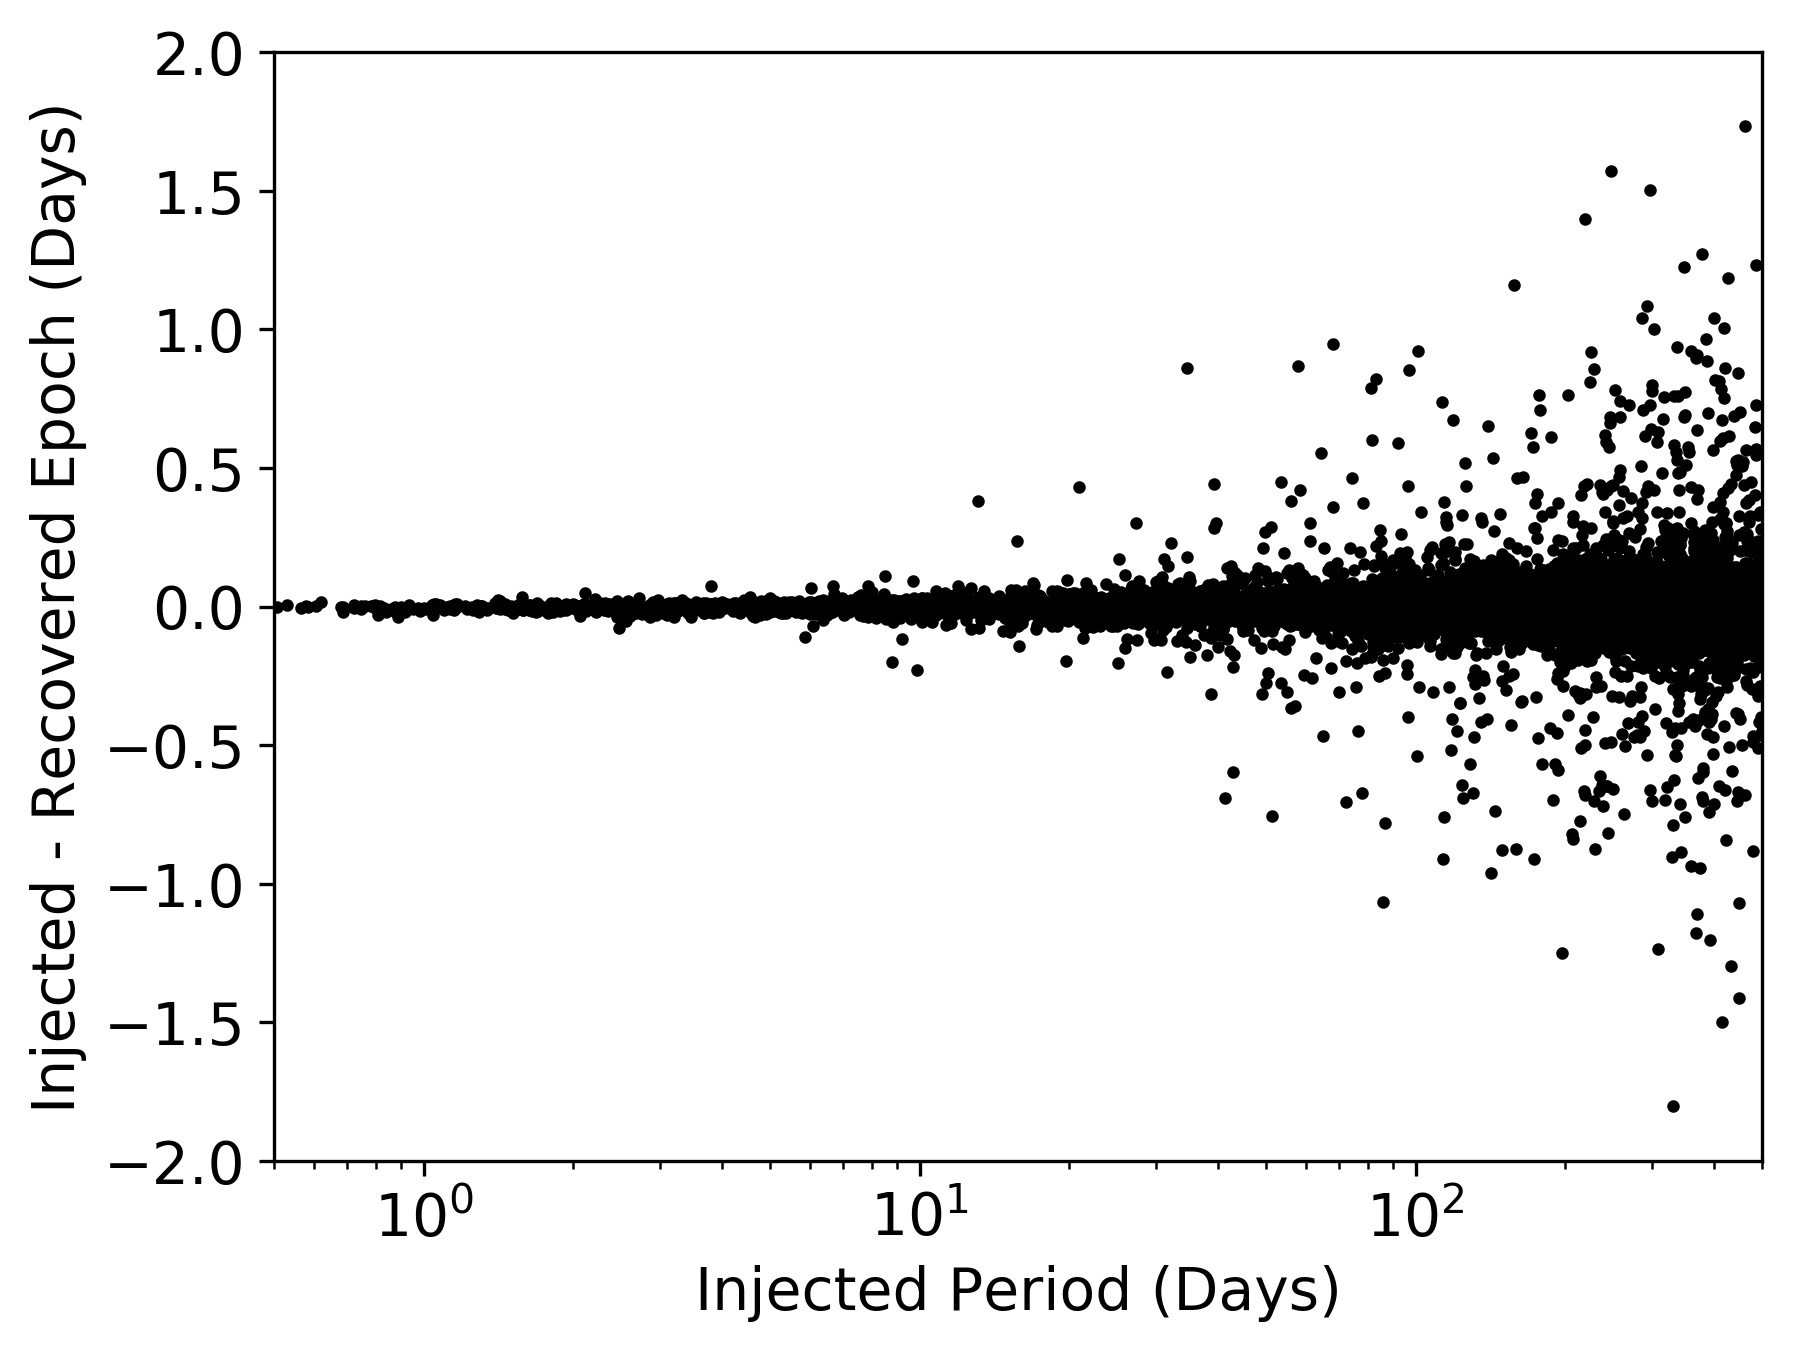
\includegraphics[width=0.5\linewidth]{INJ1-Ephem-Recovery-2.png} \\
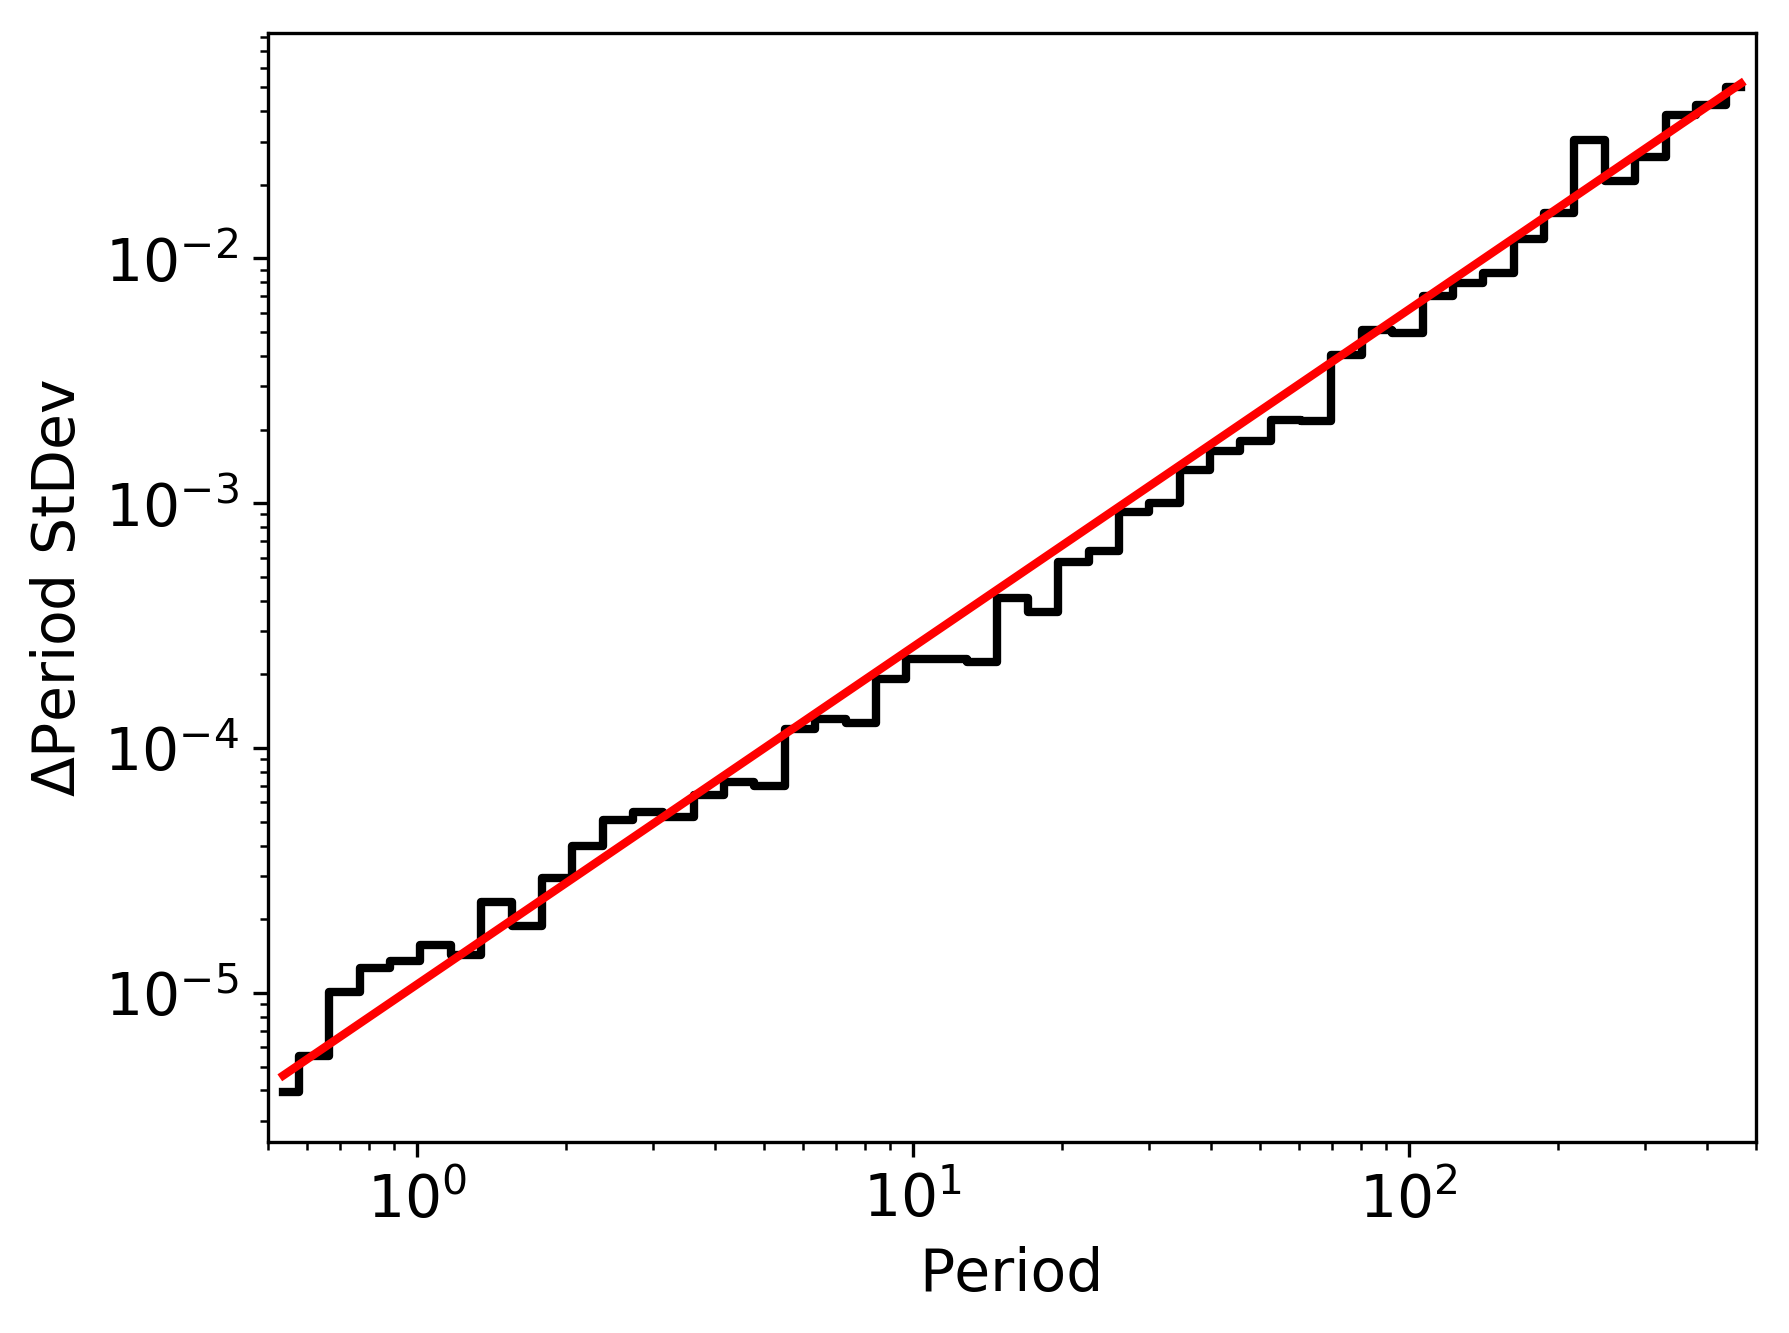
\includegraphics[width=0.5\linewidth]{INJ1-Ephem-Recovery-3.png} &
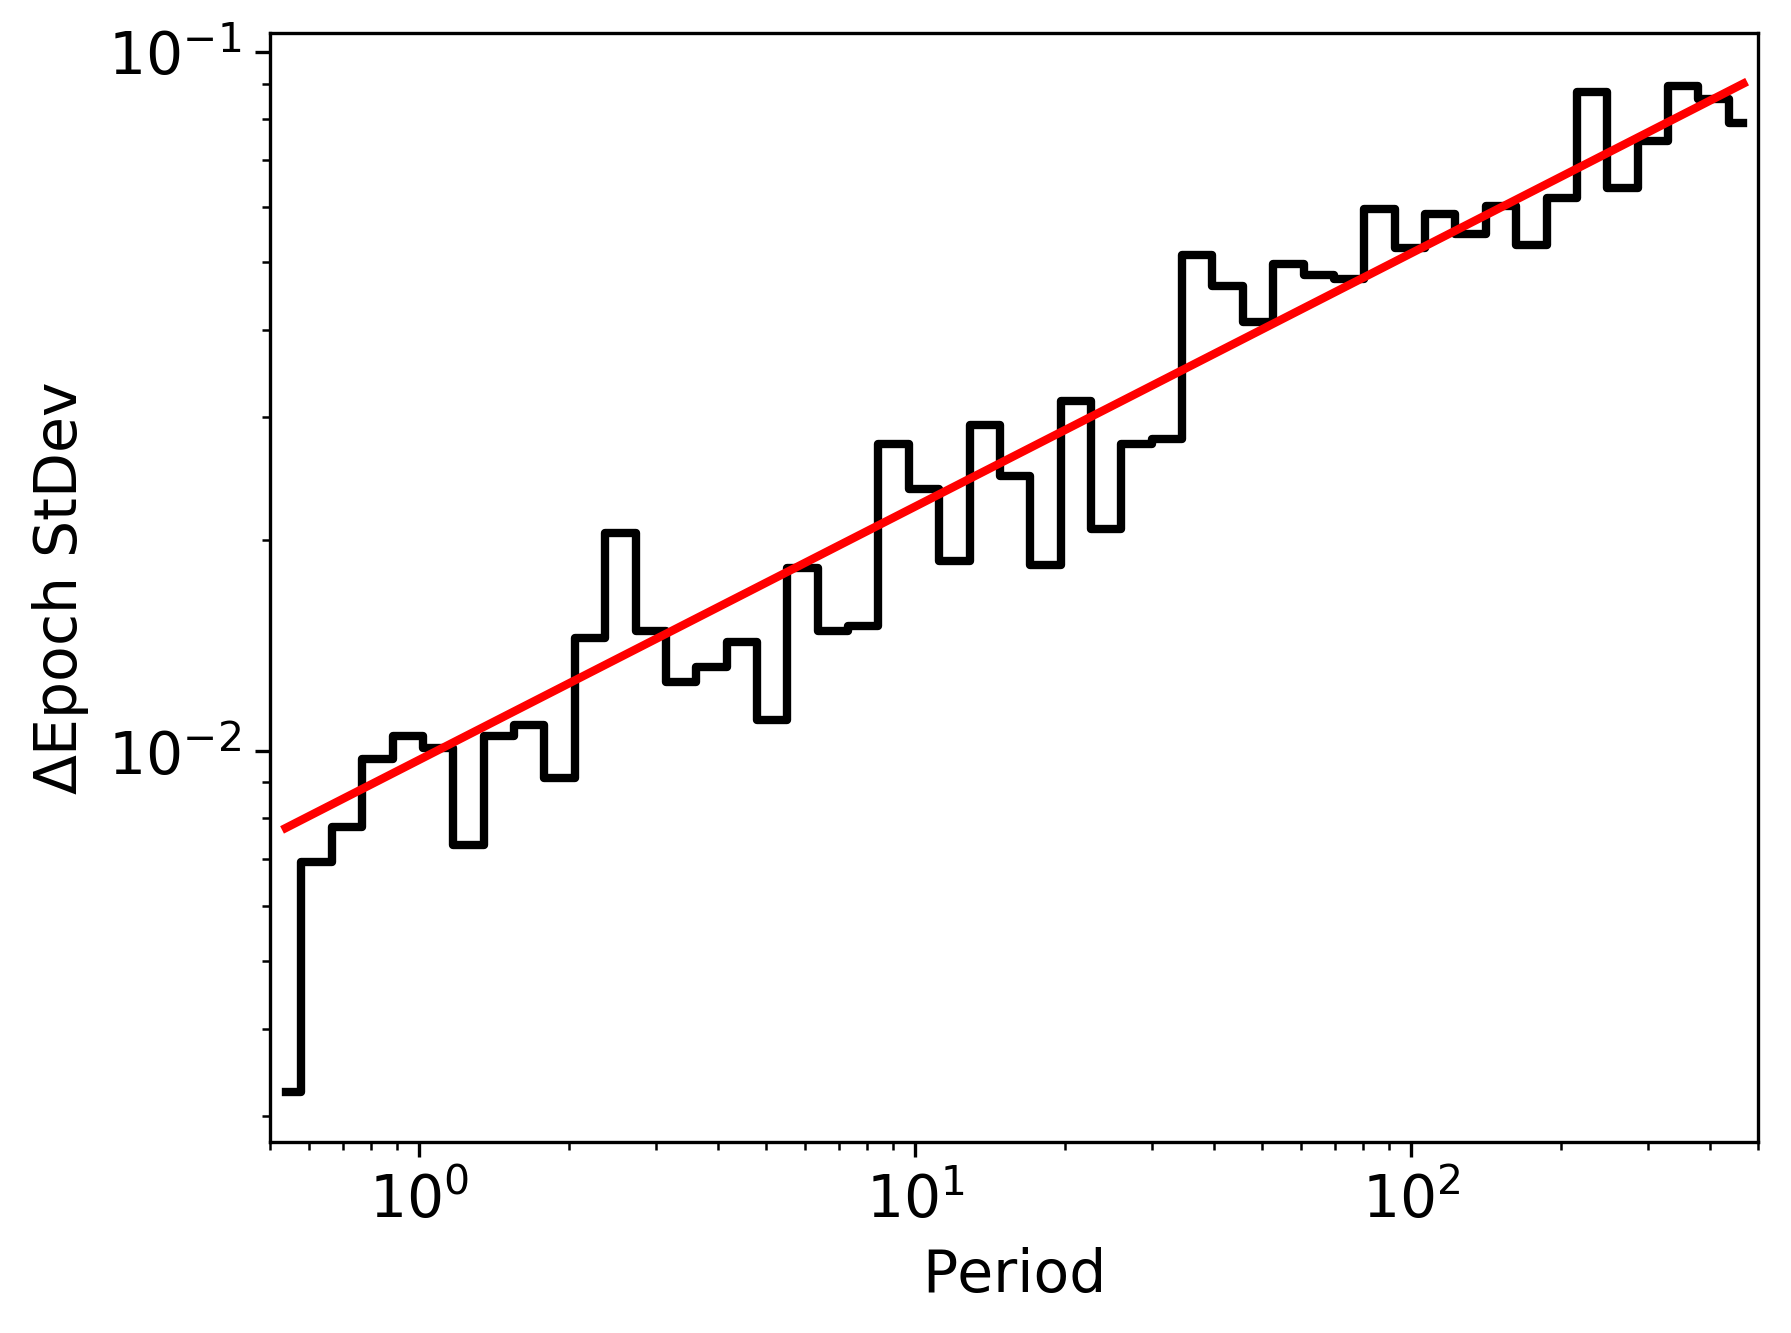
\includegraphics[width=0.5\linewidth]{INJ1-Ephem-Recovery-4.png}
\end{tabular}
\caption{A plot of injected versus recovered periods and epochs of injected on-target planets. The top plots shows the difference between the injected and recovered periods (top) and epochs (right) as a function of period. The bottom plots show the measured standard deviation of the differences in period (left) and epoch (right) in logarithmic space. The red line shows the best-fit power-law in each case.}
\label{injephemfig}
\end{figure*}


When comparing two objects, A and B, where A is defined to have the shorter period, the new matching metrics we use, $S_{P}$ and $S_{T}$ for period and epoch respectively, are:

\begin{equation}
    S_{P} = \frac{\left|P_{r} \cdot P_{A} - P_{B}\right|}{\sqrt{2}\cdot\sigma_{P}(P_{A})}
\end{equation}

\begin{equation}
    S_{T} = \frac{\left| T_{A} - T_{B} - T_{r} \cdot P_{A}\right|}{\sqrt{2}\cdot\sigma_{T}(P_{A})}
\end{equation}

\noindent where $P_{A}$ and $P_{B}$ are the periods of objects A and B, $T_{A}$ and $T_{B}$ are similarly the epochs of objects A and B, $\sigma_{P}(P_{A})$ and $\sigma_{T}(P_{A})$ are the errors in period and epoch, given period $P_{A}$, derived from the best-fit power law to the standard deviation of the injected versus recovered periods and epochs, respectively. The period ratio, $P_{r}$, and epoch ratio, $T_{r}$, are defined by:

\begin{equation}
P_{r} = \textrm{rint}\left(\frac{P_{B}}{P_{A}}\right)
\end{equation}

\begin{equation}
T_{r} = \textrm{rint}\left(\frac{T_{A} - T_{B}}{P_{A}}\right)
\end{equation}


\noindent where $\textrm{rint}()$ rounds a number to the nearest integer. Thus, a perfect match has $S_{P}$~=~0 and  $S_{T}$~=~0, with worse matches having increasingly larger values of $S_{P}$ and $S_{T}$. 

We consider matches with $S_{P}$~$<$~5 and $S_{T}$~$<$~5, with period ratios of 50 or less ($P_{r}$~$<$~50), to be statistically significant enough to constitute a match. We also require:

\begin{enumerate}

\item The two objects do not have the same KIC ID,

\item The two objects satisfy at least one of the following conditions: 

    \begin{enumerate}
    
    \item A separation distance less than $d_{\rm max}$ arcseconds, where
    \begin{equation}
    \label{disteq}
    d_{\rm max}(\arcsec) = 55\cdot\sqrt{10^{6}\cdot 10^{-0.4 \cdot m_{\rm kep}}+1}
    \end{equation}

\noindent with the \kepler{} magnitude of the brighter source being used for $m_{\rm kep}$,  

    \item Located on opposite sides of the field-of-view center, but equidistant from the center to within a 100$\arcsec$ (25 pixel) tolerance.
    
    \item Located on the same CCD module and within 5 pixels of the same column value in any of the 4 quarters.
    
    \item Located on the same CCD module and within 5 pixels of the same row and column value in any of the 4 quarters.

   \end{enumerate}

\end{enumerate}


\noindent Criterion 1 ensures that no star is ever matched to itself. Criterion 2a is a semi-empirically determined formula derived to account for direct PRF contamination and reflection off the field flattener lens, assuming the average wings of a \emph{Kepler} PSF can be approximated by a Lorentzian distribution. The formula allows for any two stars to match within a generous 55$\arcsec$ range, but allows for bright stars to match to larger distances, e.g., a 10$^{\rm th}$ mag star could match up to 550$\arcsec$ away, and a 5th mag star could match up to 5500$\arcsec$ away. Criterion 2b accounts for antipodal reflection off the Schmidt Corrector. Criterion 2c accounts for the column anomaly \citep[see \S3.5 of][]{Coughlin2016}, and criterion 2d accounts for video crosstalk.


In this Q1--Q17~DR25 catalog, we match the ephemerides of all Q1--Q17~DR25 TCEs \citep{Twicken2016}, including rogue TCEs, to the following sources:

\begin{itemize}
 \item Themselves.
 \item The list of \npredrtwentyfivekois{} KOIs from the NASA Exoplanet Archive cumulative KOI table after the closure of the Q1--Q17~DR24 table and publication of the last catalog \citep{Coughlin2016}.
 \item The \kepler{} Eclipsing Binary Working Group list of \nkebs{} ``true'' eclipsing binaries found with \kepler{} data as of 2016 October 13 \citep{Prsa2011,Slawson2011,Kirk2016}.
 \item J.M. Kreiner's up-to-date database of ephemerides of ground-based eclipsing binaries as of 2016 October 13 \citep{Kreiner2004}.
 \item Ground-based eclipsing binaries found via the TrES survey \citep{Devor2008a}.
 \item The General Catalog of Variable Stars \citep[GCVS][]{Samus2015} list of all known ground-based variable stars, published 2016 October 05.
\end{itemize}






Via ephemeris matching, we identify \nephemmatch{} Q1--Q17~DR25 TCEs as FPs. Of these, \nonlyephemmatch{} were identified as FPs only due to ephemeris matching. We list all \nephemmatch{} TCEs in Table~\ref{ephemmatchtab}, as this information is valuable for studying contamination in the \kepler{} field. In this table each TCE is identified by its KIC ID and planet number, separated by a dash. We also list in Table~\ref{ephemmatchtab} each TCE's most likely parent, the period ratio between child and parent (P$_{\rm rat}$), the distance between the child and parent in arcseconds, the offset in row and column between the child and parent in pixels ($\Delta$Row and $\Delta$Col), the magnitude of the parent (m$_{\rm Kep}$), the difference in magnitude between the child and parent ($\Delta$Mag), the depth ratio of the child and parent (D$_{\rm rat}$), the mechanism of contamination, and a flag to designate unique situations. In Figure~\ref{ephemmatchfig} we plot the location of each FP TCE and its most likely parent, connected by a solid line. TCEs are represented by solid black points, KOIs are represented by solid green points, EBs found by \kepler{} are represented by solid red points, EBs discovered from the ground are represented by solid blue points, and TCEs due to a common systematic are represented by open black points. The \kepler{} magnitude of each star is shown via a scaled point size. Most parent-child pairs are so close together that the line connecting them is not easily visible on the scale of the plot. 


\begin{deluxetable*}{ccccccccccc}
\tablecolumns{11}
\tabletypesize{\scriptsize}
\tablewidth{\linewidth}
\tablecaption{The \nephemmatch{} Q1--Q17~DR25 TCEs Identified as FPs due to Ephemeris Matches}
\tablehead{\colhead{TCE} & \colhead{Parent} & \colhead{P$_{\rm rat}$} & \colhead{Distance} & \colhead{$\Delta$Row} & \colhead{$\Delta$Col} & \colhead{m$_{\rm Kep}$} & \colhead{$\Delta$Mag} & \colhead{D$_{\rm rat}$} & \colhead{Mechanism} & \colhead{Flag} \\ & & & (\arcsec) & (Pixels) & (Pixels) & & & & & }
001433962-01 & 3924.01 & 1:1 & 13.5 & 3 & -2 & 14.91 & 0.56 & 4.7434E+02 & Direct-PRF & 0\\
001724961-01 & 001724968-01 & 1:1 & 4.7 & 1 & -1 & 13.39 & -2.96 & 2.1190E+00 & Direct-PRF & 0\\
002166206-01 & 3735.01 & 1:1 & 8.3 & -1 & -2 & 17.64 & -4.34 & 5.6706E+02 & Direct-PRF & 0\\
002309585-01 & 5982.01 & 1:1 & 11.7 & -2 & 1 & 13.93 & 1.45 & 2.0011E+02 & Direct-PRF & 0\\
002437112-01 & 3598.01 & 1:1 & 19.7 & -5 & 1 & 17.63 & -1.48 & 1.0525E+03 & Direct-PRF & 0\\
002437112-02 & 002437149-02 & 2:1 & 19.7 & -5 & 1 & 17.63 & -1.48 & 6.9253E+02 & Direct-PRF & 0\\
002437488-01 & 6268.01 & 1:1 & 10.6 & 0 & 3 & 16.98 & -2.02 & 2.5330E+02 & Direct-PRF & 0\\
002437804-01 & 002437783-01 & 1:1 & 14.4 & 4 & -1 & 17.30 & -3.14 & 1.4225E+02 & Direct-PRF & 0\\
\nodata & \nodata & \nodata & \nodata & \nodata & \nodata & \nodata & \nodata & \nodata & \nodata & \nodata\\
\enddata
\tablecomments{A suffix of ``pri'' in the parent name indicates the object is an EB known from the ground, and the child TCE matches to its primary. Similarly a suffix of ``sec'' indicates the child TCE matches the secondary of a ground-based EB. Parent names are listed, in priority order when available, by (1) their Bayer designation (e.g., RR-Lyr-pri), (2) their EBWG designation (e.g., 002449084-pri), (3) their KOI number (e.g., 3924.01), and (4) their TCE number (e.g., 001724968-01). A flag of 1 indicates that the TCE is a bastard, which are cases where two or more TCEs match each other via the Direct-PRF contamination mechanism, but neither can physically be the parent of the other via their magnitudes, depths, and distances, and thus the true parent has not been identified. A flag of 2 indicates cases of column anomalies that occur on different outputs of the same module. These cases likely involve cross-talk to carry the signal from one output to another. TCEs due to the common systematic do not have information listed for a parent source, as they are not caused by a single parent. Note that  Table~\ref{ephemmatchtab} is published in its entirety in the electronic edition of the Astrophysical Journal. A portion is shown here for guidance regarding its form and content.}
\label{ephemmatchtab}
\end{deluxetable*}


\begin{figure*}[ht]
\centering
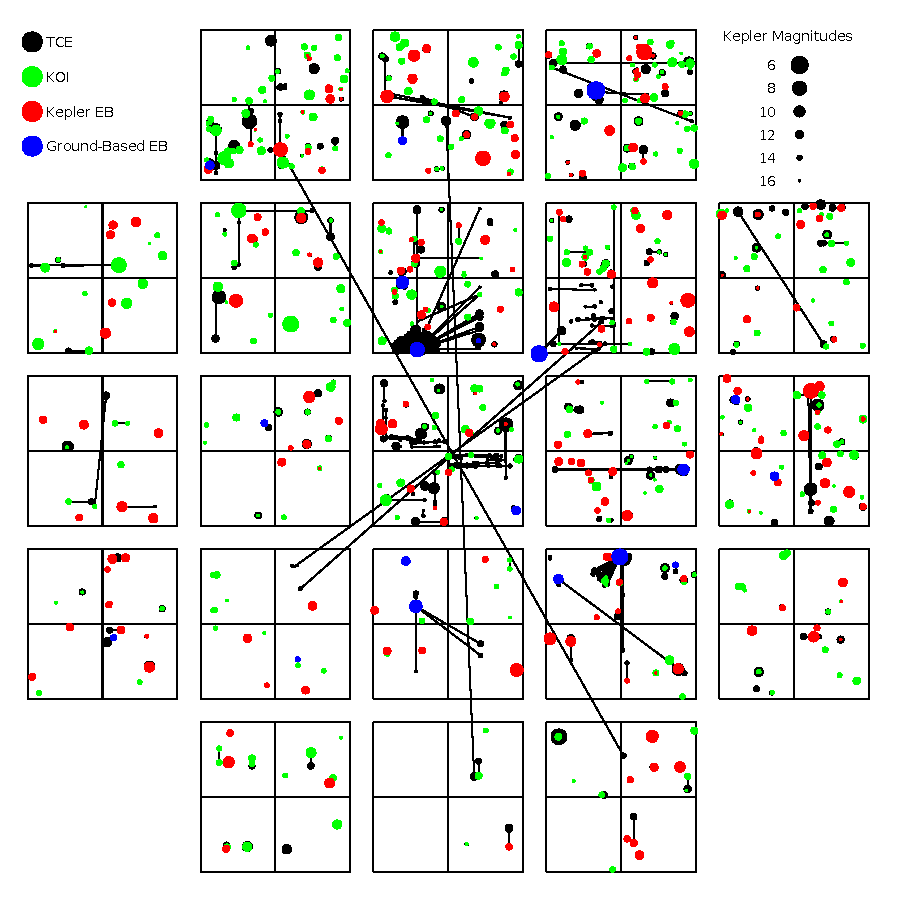
\includegraphics[width=\linewidth]{CCDPlot.pdf}
\caption{Distribution of ephemeris matches on the focal plane. Symbol size scales with magnitude, while color represents the catalog in which the contaminating source was found. Blue indicates that the true transit is from a variable star only known as a result of ground-based observations. Red circles are stars listed in the \kepler{} EBWG catalog, green are KOIs, and black are TCEs. Black lines connect false positive matches with the most likely contaminating parent. In most cases parent and child are so close that the connecting line is invisible.}
\label{ephemmatchfig}
\end{figure*}



Since \kepler{} does not observe every star in its field of view, it can often be the case that a match is found between two objects, but given their relative magnitude, distance, and depths it is clear that neither is the parent of the other, so these are classified as ``bastards'' \citep{Coughlin2014a}. To identify the bastards due to direct PRF contamination, we performed a robust fit of the Kepler PRF model described by equations~9~and~10 of \citet{Coughlin2014a} to the depth ratio, magnitude difference, and distance between each object identified as due to direct PRF contamination and its most likely parent. After iteratively rejecting outliers greater than 4.0 times the standard deviation, the fit converged with values of $\alpha$ = 6.93\arcsec and $\gamma$ = 0.358\arcsec. Outliers greater than 4.0 times the standard deviation of the final iteration, with these resulting fit parameters, were labeled as bastards. For the mechanism of column anomaly and reflection, if the depth ratio of the two objects is between 0.01 and 100, then it is labeled as a bastard, as these mechanisms should produce depth ratios of at least 1E-3 or 1E3. All bastards are identified with a flag of 1 in Table~\ref{ephemmatchtab}. Additionally, it can sometimes be the case that objects are matched via the column anomaly, but are on different outputs of the same module --- these cases likely involve the column anomaly working in conjunction with cross-talk, and thus are complicated, and given a flag of 2 in Table~\ref{ephemmatchtab}. Finally, a flag of 3 indicates a combination of flags 1 and 2. 


%Begin Jeff's words.
%Many short-period false positives are due to variable stars that exhibit a quasi-sinusoidal phased light curve. \citet{Matijevic2012} used a technique known as Local Linear Embedding (LLE), a dimensionality reduction algorithm, to classify the ``detachedness'' of \kepler{} eclipsing binary light curves on a scale of 0 to 1, where 0 represented fully detached systems with well-separated, narrow eclipses and 1 represented contact binaries with completely sinusoidal light curves. We use a similar technique, known as Local Preserving Projections \citep[][LPP]{He2004}, to distinguish transit-like signals from not transit-like signals \citep{Thompson2015b}. LPP returns a single number that represents the similarity of a TCE's shape to that of known transits. Unlike LLE, LPP can be applied to any TCE, not just those that lie within the parameter space of the training set. Thus, LPP is more suitable for separating transit-like TCEs from all other not transit-like TCEs, and can be run on artificially injected transits.


%We then fold and bin each light curve into 141 points, ensuring adequate coverage of both the in- and out-of-transit portions of the light curve. We exclude points near a phase of 0.5, as the presence of a secondary eclipse in a short-period binary may unduly influence the LPP value, and we seek to classify detached eclipsing binaries as transit-like. These 141 points act as the initial number of dimensions that describe each TCE. Using a subset of known transit-like TCEs, we create a map from the initial 141 dimensions down to 20 dimensions. We apply this map to all TCEs and measure the average Euclidean distance of each to the 15 nearest known transit-like TCEs. This average distance is the value of the LPP metric. When small, it means other transit-like TCEs are nearby in the 20 dimensional space and thus is likely to be shaped like a transit. We calculate this LPP transit metric for all TCEs using both the DV and the alternate detrending, as described in \S\ref{nottransitlikesec}.

%SUSAN - DESCRIBE HERE HOW YOU NORMALIZED THE LPP VALUES W.R.T. PERIOD, etc. 

% OLD TEXT DESCRIBING THE CHOICE OF THRESHOLD. Now we just adjust.
%
% In order to quantitatively determine a threshold between transit-like and not transit-like, we run the LPP classifier on both detrendings of the injected transits (see \S\ref{injectsec}), which we know a priori are all transit-shaped, barring any light curve distortion due to detrending. We then fit a Gaussian to the resulting distribution, computing its median and standard deviation. We then select a maximum LPP cutoff such that we expect less than one false negative in \ntces{} TCEs, via 

% \begin{equation}
% \sigma_{\rm LPP} = \sqrt{2}\cdot \textrm{erfcinv}(1/N_{\rm TCEs})
% \end{equation}

% \noindent where $N_{TCEs}$ = \ntces{}, yielding $\sigma_{\rm LPP}$ = 4.06. Any TCE with a LPP value greater than the median plus 4.06 times the standard deviation, using either detrending, is considered not transit-like.